\documentclass[12pt,a4paper,oneside]{report}             % Single-side
%\documentclass[11pt,a4paper,twoside,openright]{report}  % Duplex

%\PassOptionsToPackage{chapternumber=Huordinal}{magyar.ldf}
\usepackage{t1enc}
\usepackage[latin2]{inputenc}
\usepackage{amsmath}
\usepackage{amssymb}
\usepackage{enumerate}
\usepackage[thmmarks]{ntheorem}
\usepackage{graphics}
\usepackage{epsfig}
\usepackage{listings}
\usepackage{color}
%\usepackage{fancyhdr}
\usepackage{lastpage}
\usepackage{anysize}
\usepackage[magyar]{babel}
\usepackage{sectsty}
\usepackage{setspace}  % Ettol a tablazatok, abrak, labjegyzetek maradnak 1-es sorkozzel!
\usepackage[hang]{caption}
\usepackage{hyperref}

\usepackage{array}

%\usepackage{floatrow}SHANTI
%\usepackage{indentfirst} % Ett?l a pontok els? bekezd�se is beh�zott lesz
%\usepackage{multicol}
%\usepackage{placeins}




%--------------------------------------------------------------------------------------
% Main variables
%--------------------------------------------------------------------------------------
\newcommand{\vikszerzo}{Kiss Bal�zs}
\newcommand{\vikkonzulens}{Nagy G�bor}
%\newcommand{\vikcim}{DOKUMENTUM OSZT�LYOZ�S ADATB�NY�SZATI M�DSZEREKKEL}
\newcommand{\vikcim}{Dokumentum oszt�lyoz�s adatb�ny�szati m�dszerekkel}
\newcommand{\viktanszek}{T�vk�zl�si �s M�diainformatikai Tansz�k}
\newcommand{\vikdoktipus}{Diplomaterv}


%--------------------------------------------------------------------------------------
% Page layout setup
%--------------------------------------------------------------------------------------
% we need to redefine the pagestyle plain
% another possibility is to use the body of this command without \fancypagestyle
% and use \pagestyle{fancy} but in that case the special pages
% (like the ToC, the References, and the Chapter pages)remain in plane style

\pagestyle{plain}
%\setlength{\parindent}{0pt} % �ttekinthet?bb, angol nyelv? dokumentumokban jellemz?
%\setlength{\parskip}{8pt plus 3pt minus 3pt} % �ttekinthet?bb, angol nyelv? dokumentumokban jellemz?
\setlength{\parindent}{12pt} % magyar nyelv? dokumentumokban jellemz?
\setlength{\parskip}{0pt}    % magyar nyelv? dokumentumokban jellemz?

\marginsize{35mm}{25mm}{15mm}{15mm} % anysize package
\setcounter{secnumdepth}{0}
\sectionfont{\large\upshape\bfseries}
\setcounter{secnumdepth}{2}
\singlespacing
\frenchspacing

%--------------------------------------------------------------------------------------
%	Setup hyperref package
%--------------------------------------------------------------------------------------
\hypersetup{
    bookmarks=true,            % show bookmarks bar?
    unicode=false,             % non-Latin characters in Acrobat�s bookmarks
    pdftitle={\vikcim},        % title
    pdfauthor={\vikszerzo},    % author
    pdfsubject={\vikdoktipus}, % subject of the document
    pdfcreator={\vikszerzo},   % creator of the document
    pdfproducer={Producer},    % producer of the document
    pdfkeywords={keywords},    % list of keywords
    pdfnewwindow=true,         % links in new window
    colorlinks=true,           % false: boxed links; true: colored links
    linkcolor=black,           % color of internal links
    citecolor=black,           % color of links to bibliography
    filecolor=black,           % color of file links
    urlcolor=black             % color of external links
}

%--------------------------------------------------------------------------------------
% Set up listings
%--------------------------------------------------------------------------------------
\lstset{
	basicstyle=\scriptsize\ttfamily, % print whole listing small
	keywordstyle=\color{black}\bfseries\underbar, % underlined bold black keywords
	identifierstyle=, 					% nothing happens
	commentstyle=\color{white}, % white comments
	stringstyle=\scriptsize\sffamily, 			% typewriter type for strings
	showstringspaces=false,     % no special string spaces
	aboveskip=3pt,
	belowskip=3pt,
	columns=fixed,
	backgroundcolor=\color{lightgray},
} 		
\def\lstlistingname{lista}	

%--------------------------------------------------------------------------------------
%	Some new commands and declarations
%--------------------------------------------------------------------------------------
\newcommand{\code}[1]{{\upshape\ttfamily\scriptsize\indent #1}}

% define references
\newcommand{\figref}[1]{\ref{fig:#1}.}
\renewcommand{\eqref}[1]{(\ref{eq:#1})}
\newcommand{\listref}[1]{\ref{listing:#1}.}
\newcommand{\sectref}[1]{\ref{sect:#1}}
\newcommand{\tabref}[1]{\ref{tab:#1}.}

\DeclareMathOperator*{\argmax}{arg\,max}
%\DeclareMathOperator*[1]{\floor}{arg\,max}
\DeclareMathOperator{\sign}{sgn}
\DeclareMathOperator{\rot}{rot}
\definecolor{lightgray}{rgb}{0.95,0.95,0.95}

\author{\vikszerzo}
\title{\viktitle}
\includeonly{
	titlepage,%
	declaration,%
	abstract,%
	introduction,%
	chapter1,%
	chapter2,%
	chapter3,%
	chapter4,%
	chapter5,%
	chapter6,%
	chapter7%
}
%--------------------------------------------------------------------------------------
%	Setup captions
%--------------------------------------------------------------------------------------
\captionsetup[figure]{
%labelsep=none,
%font={footnotesize,it},
%justification=justified,
width=.75\textwidth,
aboveskip=10pt}

\renewcommand{\captionlabelfont}{\small\bf}
\renewcommand{\captionfont}{\footnotesize\it}

%--------------------------------------------------------------------------------------
% Table of contents and the main text
%--------------------------------------------------------------------------------------
\begin{document}
\singlespacing
%%--------------------------------------------------------------------------------------
% Rovid formai es tartalmi tajekoztato
%--------------------------------------------------------------------------------------

\footnotesize
\begin{center}
\large
\textbf{\Large �ltal�nos inform�ci�k, a diplomaterv szerkezete}\\
\end{center}

A diplomaterv szerkezete a BME Villamosm�rn�ki �s Informatikai Kar�n:
\begin{enumerate}
\item	Diplomaterv feladatki�r�s
\item	C�moldal
\item	Tartalomjegyz�k
\item	A diplomatervez� nyilatkozata az �n�ll� munk�r�l �s az elektronikus adatok kezel�s�r�l
\item	Tartalmi �sszefoglal� magyarul �s angolul
\item	Bevezet�s: a feladat �rtelmez�se, a tervez�s c�lja, a feladat indokolts�ga, a diplomaterv fel�p�t�s�nek r�vid �sszefoglal�sa
\item	A feladatki�r�s pontos�t�sa �s r�szletes elemz�se
\item	El�zm�nyek (irodalomkutat�s, hasonl� alkot�sok), az ezekb�l levonhat� k�vetkeztet�sek
\item	A tervez�s r�szletes le�r�sa, a d�nt�si lehet�s�gek �rt�kel�se �s a v�lasztott megold�sok indokl�sa
\item	A megtervezett m�szaki alkot�s �rt�kel�se, kritikai elemz�se, tov�bbfejleszt�si lehet�s�gek
\item	Esetleges k�sz�netnyilv�n�t�sok
\item	R�szletes �s pontos irodalomjegyz�k
\item	F�ggel�k(ek)
\end{enumerate}

Felhaszn�lhat� a k�vetkez� oldalt�l kezd�d� \LaTeX-Diplomaterv sablon dokumentum tartalma. 

A diplomaterv szabv�nyos m�ret� A4-es lapokra ker�lj�n. Az oldalak t�k�rmarg�val k�sz�ljenek (mindenhol 2.5cm, baloldalon 1cm-es k�t�ssel). Az alap�rtelmezett bet�k�szlet a 12 pontos Times New Roman, m�sfeles sork�zzel.

Minden oldalon - az els� n�gy szerkezeti elem kiv�tel�vel - szerepelnie kell az oldalsz�mnak.

A fejezeteket decim�lis beoszt�ssal kell ell�tni. Az �br�kat a megfelel� helyre be kell illeszteni, fejezetenk�nt decim�lis sz�mmal �s kifejez� c�mmel kell ell�tni. A fejezeteket decim�lis al�oszt�ssal sz�mozzuk, maxim�lisan 3 al�oszt�s m�lys�gben (pl. 2.3.4.1.). Az �br�kat, t�bl�zatokat �s k�pleteket c�lszer� fejezetenk�nt k�l�n sz�mozni (pl. 2.4. �bra, 4.2 t�bl�zat vagy k�pletn�l (3.2)). A fejezetc�meket igaz�tsuk balra, a norm�l sz�vegn�l viszont haszn�ljunk sorkiegyenl�t�st. Az �br�kat, t�bl�zatokat �s a hozz�juk tartoz� c�met igaz�tsuk k�z�pre. A c�m a jel�lt r�sz alatt helyezkedjen el.

A k�peket lehet�leg rajzol� programmal k�sz�ts�k el, az egyenleteket egyenlet-szerkeszt� seg�ts�g�vel �rj�k le (A \LaTeX~ehhez k�zenfekv� megold�sokat ny�jt).

Az irodalomjegyz�k sz�vegk�zi hivatkoz�sa t�rt�nhet a Harvard-rendszerben (a szerz� �s az �vsz�m megad�s�val) vagy sorsz�mozva. A teljes lista n�vsor szerinti sorrendben a sz�veg v�g�n szerepeljen (sorsz�mozott irodalmi hivatkoz�sok eset�n hivatkoz�si sorrendben). A szakirodalmi forr�sok c�meit azonban mindig az eredeti nyelven kell megadni, esetleg z�r�jelben a ford�t�ssal. A list�ban szerepl� valamennyi publik�ci�ra hivatkozni kell a sz�vegben (a \LaTeX-sablon a Bib\TeX~seg�ts�g�vel mindezt automatikusan kezeli). Minden publik�ci� a szerz�k ut�n a k�vetkez� adatok szerepelnek: foly�irat cikkekn�l a pontos c�m, a foly�irat c�me, �vfolyam, sz�m, oldalsz�m t�l-ig. A foly�irat c�meket csak akkor r�vid�ts�k, ha azok nagyon k�zismertek vagy nagyon hossz�ak. Internet hivatkoz�sok megad�sakor fontos, hogy az el�r�si �t el�tt megadjuk az oldal tulajdonos�t �s tartalm�t (mivel a link egy id� ut�n ak�r el�rhetetlenn� is v�lhat), valamint az el�r�s id�pontj�t.

\vspace{5mm}
Fontos:
\begin{itemize}
	\item A szakdolgozat k�sz�t� / diplomatervez� nyilatkozata (a jelen sablonban szerepl� sz�vegtartalommal) k�telez� el��r�s Karunkon ennek hi�ny�ban a szakdolgozat/diplomaterv nem b�r�lhat� �s nem v�dhet� !
	\item Mind a dolgozat, mind a mell�klet maxim�lisan 15 MB m�ret� lehet !
\end{itemize}

\vspace{5mm}
\begin{center}
J� munk�t, sikeres szakdolgozat k�sz�t�st ill. diplomatervez�st k�v�nunk !
\end{center}

\normalsize

%%--------------------------------------------------------------------------------------
% Feladatkiiras (a tanszeken atveheto, kinyomtatott valtozat)
%--------------------------------------------------------------------------------------
\clearpage
\begin{center}
\large
\textbf{FELADATKI�R�S}\\
\end{center}

A feladatki�r�st a tansz�ki adminisztr�ci�ban lehet �tvenni, �s a leadott munk�ba eredeti, tansz�ki pecs�ttel ell�tott �s a tansz�kvezet� �ltal al��rt lapot kell belef�zni (ezen oldal \emph{helyett}, ez az oldal csak �tmutat�s). Az elektronikusan felt�lt�tt dolgozatban m�r nem kell beleszerkeszteni ezt a feladatki�r�st.

\begin{center}
\LARGE
\color{red}\textbf{EZ AZ OLDAL NE LEGYEN BENNE A DIGIT�LISBAN, NYOMTATOTTBAN IDE KELL BEK�TNI A TANSZ�KR�L �TVETT FELADATKI�R�ST}
\end{center}





\pagenumbering{arabic}
\onehalfspacing
%--------------------------------------------------------------------------------------
%	The title page
%--------------------------------------------------------------------------------------
\begin{titlepage}
\begin{center}

\includegraphics[width=60mm,keepaspectratio]{figures/BMElogo.png}\\
\vspace{0.3cm}
\textbf{Budapesti M�szaki �s Gazdas�gtudom�nyi Egyetem}\\
\textmd{Villamosm�rn�ki �s Informatikai Kar}\\
\textmd{\viktanszek}\\[5cm]

\vspace{0.4cm}
{\huge \bfseries \vikcim}\\[0.8cm]
\vspace{0.5cm}
\textsc{\Large \vikdoktipus}\\[4cm]

\begin{tabular}{cc}
 \makebox[7cm]{\emph{K�sz�tette}} & \makebox[7cm]{\emph{Konzulens}} \\
 \makebox[7cm]{\vikszerzo} & \makebox[7cm]{\vikkonzulens}
\end{tabular}

\vfill
{\large \today}
\end{center}
\end{titlepage}



\tableofcontents\vfill
%--------------------------------------------------------------------------------------
% Nyilatkozat
%--------------------------------------------------------------------------------------
\begin{center}
\large
\textbf{HALLGAT�I NYILATKOZAT}\\
\end{center}

Alul�rott \emph{\vikszerzo}, szigorl� hallgat� kijelentem, hogy ezt a szakdolgozatot/ diplomatervet \textcolor{blue}{(nem k�v�nt t�rlend�)} meg nem engedett seg�ts�g n�lk�l, saj�t magam k�sz�tettem, csak a megadott forr�sokat (szakirodalom, eszk�z�k stb.) haszn�ltam fel. Minden olyan r�szt, melyet sz� szerint, vagy azonos �rtelemben, de �tfogalmazva m�s forr�sb�l �tvettem, egy�rtelm�en, a forr�s megad�s�val megjel�ltem.

Hozz�j�rulok, hogy a jelen munk�m alapadatait (szerz�(k), c�m, angol �s magyar nyelv� tartalmi kivonat, k�sz�t�s �ve, konzulens(ek) neve) a BME VIK nyilv�nosan hozz�f�rhet� elektronikus form�ban, a munka teljes sz�veg�t pedig az egyetem bels� h�l�zat�n kereszt�l (vagy autentik�lt felhaszn�l�k sz�m�ra) k�zz�tegye. Kijelentem, hogy a beny�jtott munka �s annak elektronikus verzi�ja megegyezik. D�k�ni enged�llyel titkos�tott diplomatervek eset�n a dolgozat sz�vege csak 3 �v eltelte ut�n v�lik hozz�f�rhet�v�.

\begin{flushleft}
\vspace*{1cm}
Budapest, \today
\end{flushleft}

\begin{flushright}
 \vspace*{1cm}
 \makebox[7cm]{\rule{6cm}{.4pt}}\\
 \makebox[7cm]{\emph{\vikszerzo}}\\
 \makebox[7cm]{hallgat�}
\end{flushright}
\thispagestyle{empty}

\vfill
\clearpage
\thispagestyle{empty} % an empty page


%----------------------------------------------------------------------------
% Abstract in hungarian
%----------------------------------------------------------------------------
\chapter*{Kivonat}\addcontentsline{toc}{chapter}{Kivonat}

Jelen dokumentum egy diplomaterv sablon, amely formai keretet ad a BME Villamosm�rn�ki �s Informatikai Kar�n v�gz� hallgat�k �ltal elk�sz�tend� szakdolgozatnak �s diplomatervnek. A sablon haszn�lata opcion�lis. Ez a sablon \LaTeX~alap�, a \emph{TeXLive} \TeX-implement�ci�val �s a PDF-\LaTeX~ford�t�val m�k�d�k�pes.
\vfill

%----------------------------------------------------------------------------
% Abstract in english
%----------------------------------------------------------------------------
\chapter*{Abstract}\addcontentsline{toc}{chapter}{Abstract}

This document is a \LaTeX-based skeleton for BSc/MSc~theses of students at the Electrical Engineering and Informatics Faculty, Budapest University of Technology and Economics. The usage of this skeleton is optional. It has been tested with the \emph{TeXLive} \TeX~implementation, and it requires the PDF-\LaTeX~compiler.
\vfill


%----------------------------------------------------------------------------
\chapter*{Bevezet�}\addcontentsline{toc}{chapter}{Bevezet�}
%----------------------------------------------------------------------------

A bevezet� bevezet� BEVEZET? tartalmazza a diplomaterv-ki�r�s elemz�s�t, t�rt�nelmi el�zm�nyeit, a feladat indokolts�g�t (a motiv�ci� le�r�s�t), az eddigi megold�sokat, �s ennek t�kr�ben a hallgat� megold�s�nak �sszefoglal�s�t.

A bevezet� szok�s szerint a diplomaterv fel�p�t�s�vel z�r�dik, azaz annak r�vid le�r�s�val, hogy melyik fejezet mivel foglalkozik.


%----------------------------------------------------------------------------
\chapter{\LaTeX-eszk�z�k}\label{sect:LatexTools}
%----------------------------------------------------------------------------
\section{A szerkeszt�shez haszn�latos, Windows alap� eszk�z�k}
%----------------------------------------------------------------------------
Ez a sablon Windows oper�ci�s rendszer alatt k�sz�lt TeXnicCenter 1 Beta 7.01 szerkeszt�vel. A TeXnicCenter egy \LaTeX-szerkeszt�program sz�mtalan hasznos -- �s r�ad�sul j�l m�k�d� -- szolg�ltat�ssal (\figref{TexnicCenter} �bra). A szoftver ingyenesen let�lthet� a\\\url{http://www.texniccenter.org/} c�mr�l.

\begin{figure}[!ht]
\centering
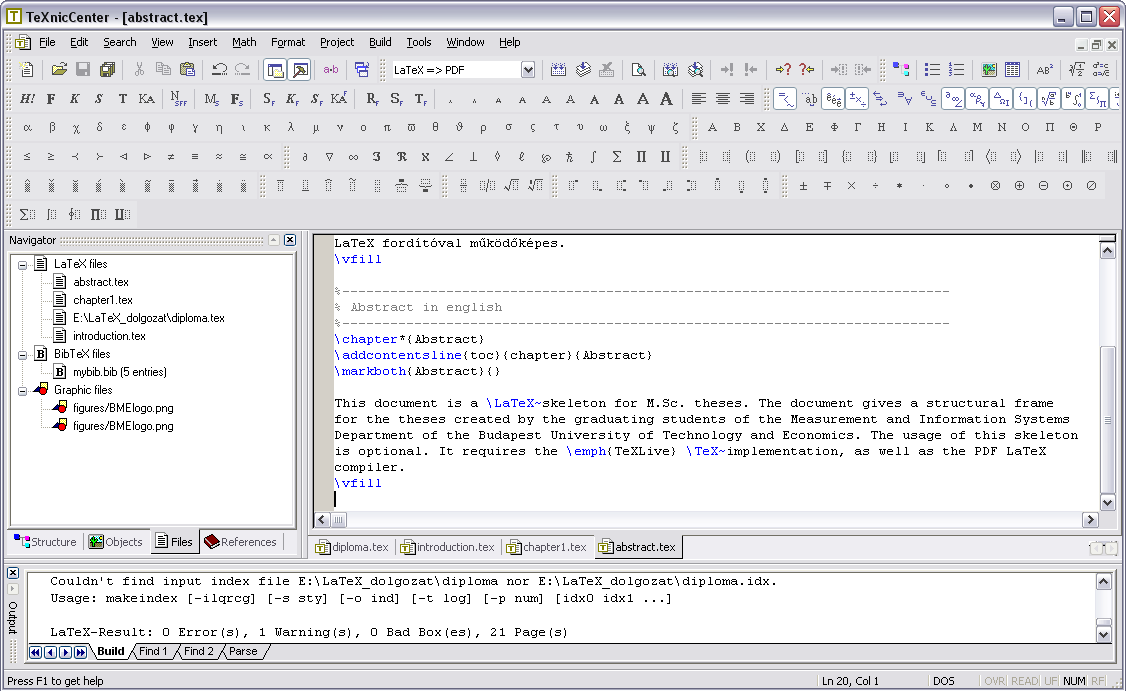
\includegraphics[width=150mm, keepaspectratio]{figures/TeXnicCenter.png}
\caption{A TeXnicCenter Windows alap� \LaTeX-szerkeszt�.} 
\label{fig:TexnicCenter}
\end{figure}

Egy m�sik haszn�lhat� Windows alap� szerkeszt�program a LEd (LaTeX Editor,\\\url{http://www.latexeditor.org/}), a TeXnicCenter azonban stabilabb, gyorsabb, �s jobban haszn�lhat�.

%----------------------------------------------------------------------------
\section{A dokumentum leford�t�sa Windows alatt}
%----------------------------------------------------------------------------
A TeXnicCenter �s a LEd kiz�r�lag szerkeszt�program (b�r az ut�bbiban DVI-n�zeget� is van), �gy a dokumentum ford�t�s�hoz sz�ks�ges eszk�z�ket nem tartalmazza. Windows alatt alapvet�en k�t lehet�s�g k�z�l �rdemes v�lasztani: MiKTeX (\url{http://miktex.org/}) �s TeXLive (\url{http://www.tug.org/texlive/}) programcsomag. Az ut�bbi m�k�dik Mac OS X, GNU/Linux alatt �s Unix-sz�rmaz�kokon is. A MiKTeX egy alapcsomag telep�t�se ut�n mindig let�lti a haszn�lt funkci�khoz sz�ks�ges, de lok�lisan hi�nyz� \TeX-csomagokat, m�g a TeXLive DVD ISO verz�ban f�rhet� hozz�. Ez a dokumentum TeXLive 2008 programcsomag seg�ts�g�vel fordult, amelynek DVD ISO verzi�ja a megadott oldalr�l let�lthet�. A sablon leford�t�s�hoz a disztrib�ci�ban szerepl� \verb+magyar.ldf+ f�jlt a \verb+http://www.math.bme.hu/latex/+ v�ltozatra kell cser�lni, vagy az ut�bbi v�ltozatot be kell m�solni a projekt-k�nyvt�rba (ahogy ezt meg is tett�k a sablonban) k�l�nben anom�li�k tapasztalhat�k a dokumentumban (pl. az �bra- �s t�bl�zat-al��r�sok form�tuma nem a be�ll�tott lesz, vagy bizonyos oldalakon megjelenik alap�telmez�sben egy fejl�c). A TeXLive 2008-at m�g nem kell k�l�n telep�teni a g�pre, elegend� DVD-r�l (vagy az ISO f�jlb�l k�zvetlen�l, pl. DaemonTools-szal) haszn�lni. 

A \TeX-eszk�z�ket tartalmaz� programcsomag bin�risainak el�r�si �tj�t minden esetben be kell �ll�tani a szerkeszt�programban, p�ld�ul TeXnicCenter eset�n legegyszer�bben a \verb+Build / Define output profiles...+ men�ponttal el�h�vott dial�gusablakban a \verb+Wizard...+ gombra kattintva tehetj�k ezt meg.

A PDF-\LaTeX~haszn�lata eset�n a gener�lt dokumentum k�zvetlen�l PDF-form�tumban �ll rendelkez�sre. Amennyiben a PDF-f�jl egy PDF-n�z�ben (pl. Adobe Acrobat Reader vagy Foxit PDF Reader) meg van nyitva, akkor a f�jlle�r�t a PDF-n�z� program tipikusan lefoglalja. Ilyen esetben a dokumentum �jraford�t�sa hiba�zenettel kil�p. Ha bez�rjuk �s �jra megnyitjuk a PDF dokumentumot, akkor pedig a PDF-n�z�k t�bbs�ge az els� oldalon nyitja meg a dokumentumot, nem a legut�bb olvasott oldalon. Ezzel szemben p�ld�ul az egyszer� �s ingyenes \textcolor{blue}{Sumatra PDF} nev� program k�pes arra, hogy a megnyitott dokumentum megv�ltoz�s�t detekt�lja, �s friss�tse a n�zetet az aktu�lis oldal megtart�s�val.

%----------------------------------------------------------------------------
\section{Eszk�z�k Linuxhoz}
%----------------------------------------------------------------------------
Linux oper�ci�s rendszer alatt is rengeteg szerkeszt�program van, pl. a KDE alap� Kile j�l haszn�lhat�. Ez ingyenesen let�lthet�, vagy �ppens�ggel az adott Linux-disztrib�ci� eleve tartalmazza, ahogyan a dokumentum ford�t�s�hoz sz�ks�ges csomagokat is. Az Ubuntu Linux disztrib�ci�k alatt p�ld�ul legt�bbsz�r a \verb+texlive-base+ csomag telep�t�s�vel haszn�lhat�k a \LaTeX-eszk�z�k.

%----------------------------------------------------------------------------
\chapter{Felhaszn�lt webes technol�gi�k}\label{sect:usedWebTechs}
%----------------------------------------------------------------------------
A feladatom sor�n nagyban �p�tkeztem a kor�bbi �n�ll� laborat�rium sor�n megismert technol�gi�kra. Seg�ts�g�kkel b�v�tettem a kor�bbi megold�st, �s implement�ltam �j elj�r�sokat, melyhez sz�ks�gem volt �j technol�gi�k megismer�s�re.  

A feladat megold�s�hoz egy olyan k�nnyen konfigur�lhat�, sokr�t� webalkalmaz�s elk�sz�t�s�re t�rekedtem, amely b�v�thet�, k�nnyed�n be�p�thet� a k�s�bbiekben m�s rendszerekbe, illetve term�szetesen az adat- �s sz�vegb�ny�szati modulok is integr�lhat�ak legyenek bele. A v�lasztott keretrendszer �gy a Python nyelvre �r�dott framework \cite{WebFramework}, a Django\cite{django} lett.
%----------------------------------------------------------------------------
\section{Python}
%----------------------------------------------------------------------------
A Python\cite{pythonBook} egy �ltal�nos c�l�, magas szint� programoz�si nyelv. Elterjed�s�nek okai t�bbek k�z�tt a j� felhaszn�lhat�s�g, j� fut�sid�-optimaliz�ci�, eleg�ns megold�sok �s olvashat� k�dk�p. �n a Python 3.3.3-as verzi�j�t haszn�ltam a feladat megval�s�t�s�ra. 

A nyelv objektumorient�lt, ingyenesen haszn�lhat�, m�k�dik a legt�bb modern oper�ci�s rendszer felett. Scriptek �r�s�t�l a komplex, t�bbr�teg� alkalmaz�sok implement�l�s�ig haszn�lhat�. 

K�dk�pe t�m�r �s j�l olvashat�: szok�sos programoz�si konvenci�kt�l t�bb helyen is elt�r az egyszer�s�g �s �tl�that�s�g c�lj�b�l. A k�dban a sort�r�s kiv�ltja a pontosvessz�k haszn�lat�t az utas�t�sok lez�r�s�hoz, illetve a k�dblokkok elv�laszt� elemei a bekezd�sek, a szok�sos kapcsos z�r�jelek helyett. 

\begin{lstlisting}[frame=single,caption=A Fibonacci sz�mok kisz�mol�sa Python nyelven, label=pythonfibo, float=!ht]
>>> def fib(n):
>>>     a, b = 0, 1
>>>     while a < n:
>>>         print(a, end=' ')
>>>         a, b = b, a+b
>>>     print()
>>> fib(1000)
\end{lstlisting}

Automatikus, �s effekt�v er�forr�s kezel�st val�s�t meg, adatt�pusai magasan fejlettek. Pointerek haszn�lata egy�ltal�n nincs. K�nnyed�n t�bbsz�l�s�that�, �s j�l interpret�lt, compile m�d� m�k�d�se is lehets�ges. Ma m�r sz�les fejleszt�i k�z�ss�g munk�lkodik m�g�tte, melynek k�sz�nhet�en folyamatosan fejl�dik.
%----------------------------------------------------------------------------
\section{Webalkalmaz�sok}
%----------------------------------------------------------------------------
A feladathoz megalkotott szoftverem egyik jellemz�je, hogy webes alkalmaz�sk�nt el�rhet� a szabv�nyos b�ng�sz�k seg�ts�g�vel.

A szoftver felhaszn�l� fel�lete �gy gener�lt HTML weblapokb�l �ll, melyeket egy webszerver �ll�t el�. Ez a webszerver felel�s az alkalmaz�s �zleti logik�j�nak futtat�s��rt, a webes k�r�sek kiszolg�l�s��rt, megjelen�tend� weboldalak el��ll�t�s��rt �s az �rkez� http k�r�sek kiszolg�l�s��rt.

A webszerver HTTP \cite{httpRFC} felett k�l�nb�z� csomagokat k�ld �s fogad. A k�r�seknek k�t kateg�ri�j�t haszn�ltam fel:

\begin{itemize}
	\item \textbf{GET}: a kliens oldal�r�l �rkez� http request csomag, mely valamilyen adat lek�rdez�s�re ir�nyul legt�bbsz�r (RESTful\cite{restful} web service eset�ben). P�ld�ul az egyes linkekre val� kattint�s, vagy gombok lenyom�sa.
	\item \textbf{POST}: a kliens oldal�r�l �rkez�, szint�n http request t�pus, amely valamilyen adatot k�ld feldolgoz�s c�lj�ra. A felhaszn�l� a feladatom sor�n, a webes fel�leten adhatja meg azt a sz�veget, linkeket, melyekre szeretn� futtatni az elemz�si elj�r�sokat. Az inform�ci�t egy POST �zenetben k�ldi el a szerver sz�m�ra, mely azt tov�bb�tja az adatb�ny�szati modul fel�. 
\end{itemize}


%----------------------------------------------------------------------------
\section{Django}
%----------------------------------------------------------------------------
A Django egy Python webalkalmaz�s keretrendszer. A t�bbi keretrendszerhez hasonl�an, egy m�r megval�s�tott, gyakran �jrafelhaszn�lt oszt�lyokat tartalmaz� csomag, mely seg�ts�g�vel nem kell null�r�l elkezden�nk egy webalkalmaz�s meg�r�s�t. 

\begin{figure}[!ht]
	\centering
	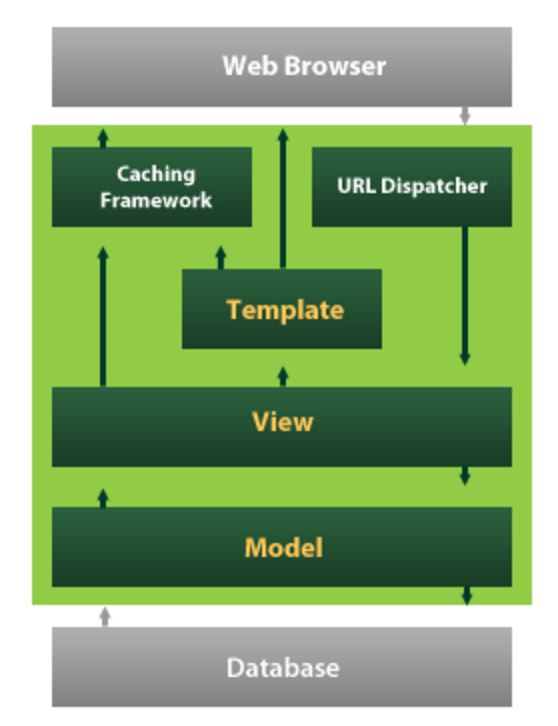
\includegraphics[width=70mm, keepaspectratio]{figures/DjangoArch.png}
	\caption{Django architekt�ra\cite{djangoArch}} 
	\label{DjangoArch}
\end{figure}

Az alkalmaz�s Model-View-Controller \cite{mvcArch} alapokra t�maszkodik �s f� c�lja az �j webalkalmaz�sok egyszer� l�trehoz�sa: az el�re meghat�rozott �p�t�elemek seg�ts�g�vel percek alatt k�pesek vagyunk egy m�k�d� webszervert ind�tani, rajta a telep�tett alkalmaz�sunkkal, mely �gy k�pes webes k�r�sek kiszolg�l�s�ra, websevice-ek \cite{webservice} �zemeltet�s�re.

\Aref{DjangoArch} �br�n l�that� a szoftver �ltal�nos szerkezete. Az adatb�zis �s a model k�z�tti szinkroniz�ci� automatikus. A view r�teg dolgozza fel a be�rkez� k�r�seket, sz�l�tja meg a bels� �zleti logik�t (ami a mostani esetben az adatb�ny�szati modul f�ggv�nyei), kommunik�l az adatb�zissal. Ebb�l a h�rmasb�l �ll�tja el� az el�re defini�lt weboldal-template-ek kieg�sz�t�s�vel a megjelen�tend� weboldalt. 

Egy tipikus weboldal l�trehoz�sa a k�vetkez� l�p�sekb�l �llhat:
\begin{enumerate}
	\item Architekt�ra, k�nyvt�rszerkezet kialak�t�sa. A manage.py param�terez�s�vel k�nnyed�n kialak�that� egy el�zetes k�nyvt�rszerkezet, a k�l�nb�z� r�tegeknek megfelel�en. Az alkalmaz�s v�z�nak l�trehoz�sakor m�r k�pesek vagyunk elind�tani az webszervert, kiszolg�lni a k�r�seket, adminisztr�tori fel�leten bel�pni, felhaszn�l�kat menedzselni: teh�t a leggyakoribb feladatokhoz megkapjuk a keretet.
	\item Model defini�l�s. A keretrendszer seg�ts�g�vel el�re meghat�rozott m�don tudunk model objektumokat l�trehozni, melyekek el�re gener�lt megjelen�t� fel�letekkel rendelkeznek. A feladatom sor�n olyan dokumentum objektumokat hoztam l�tre, melyek ilyen m�don m�r el�re rendelkeztek a hozz�juk tartoz� megfelel� model form-mal, �s ig�ny szerint ak�r adatb�zis perziszt�l�ssal is.
	\item 	URL-ek megad�sa: a weboldalak bek�t�s�re k�l�n fel�let �ll rendelkez�sre, ahol az egyes k�r�sek bel�p�si pontjait �s a v�lasz oldalak el�rhet�s�g�t �ll�thatjuk be.
	\item Template-ek l�trehoz�sa. A webes megjelen�t� fel�letre egy saj�t template nyelv seg�ts�g�vel lehet defini�lni a k�s�bbiekben legener�land�, statikus �s dinamikus tartalommal rendelkez� oldalakat.
	\item Control r�teg. Itt �r �ssze az �tvonalak �s k�r�sek kiszolg�l�sa. A be�rkez� GET �s POST http k�r�sekre az �zleti logik�t felhaszn�lva v�laszokat �ll�tunk el�, amelyeket a template-ek, �s a benn�k tal�lhat� dinamikus v�ltoz�k behelyettes�t�s�vel hozunk l�tre.
\end{enumerate}

Term�szetesen ez csak egy fel�letes �ttekint�se a keretrendszerben rejl� lehet�s�geknek: a feladatom megold�s�hoz az itt felsorolt lehet�s�gek elegend�nek is bizonyultak az adatb�ny�szati modul felhaszn�l�s�hoz, annak megjelen�t�s�hez.

%----------------------------------------------------------------------------
\section{Beautiful Soup}
%----------------------------------------------------------------------------

A Beautiful Soup \cite{BeautifulSoup} egy Python libary, amit web parse feladatok(azaz weboldal tartalom kinyer�s�nek) k�nny� megval�s�t�s�hoz terveztek.

F� feladata, hogy k�pes egyszer� navig�ci�s l�p�sekre weboldalak lek�r�s�hez. 
A lek�rdezett weboldalak dokumentum alap� tartalm�t egy bels� fa adatszerkezetben t�rolja, melyen k�l�nb�z� feldolgoz�si l�p�seket lehet megval�s�tani.

T�mogatja a tartalmak felolvas�s�t, k�nny� �s egyszer� szintaktik�ja seg�ts�g�vel gyorsan el�rhetj�k az XML f�jlok sz�munkra �rdekes r�szeit. Unicode k�dol�st t�mogatva ide�lis magyar nyelv� sz�vegek kinyer�s�re is.

Er�ss�ge abban rejlik, hogy azon parser-eken fel�l, amelyre �p�tkezik (lxml, html5lib), el�re defini�lt bej�r�si eszk�z�kkel is rendelkezik, teh�t ezt nem nek�nk kell megval�s�tani. Ez ut�bbi tulajdons�ga egyes dokumentumfa bej�r�si feladatokn�l nagyon hasznos.

Az el�zetes kutat�s sor�n ezt az eszk�zt haszn�ltam t�bbek k�z�tt a weboldalak, �s azok RSS feed-j�nek \cite{XmlDesc} lek�r�s�re, ebb�l a linkek kiv�logat�s�ra. A linkek m�g�tt rejl� weboldalak sz�veg�t is ennek az eszk�znek a seg�ts�g�vel �rtem el. 
P�ld�ul egy weboldalra mutat� url-b�l \aref{URLParse} k�dr�szleten l�that� m�don tudjuk kinyerni a sz�veg c�m�t.

\begin{lstlisting}[frame=single, caption=URL parse-ol�sa, label=URLParse,  float=!ht]
def parse_title(urlText):
resp = requests.get(urlText)
soup = BeautifulSoup(resp.text)
return soup.find('h1').text	
\end{lstlisting}

Els� l�p�sben a resp objektumban let�rolja a lek�rdezett HTML oldalt. A soup objektum t�rolja a HTML oldal sz�veg r�sz�t, a felesleges metaadatok n�lk�l, a m�r eml�tett fa form�tumban. A find f�ggv�ny visszat�r a HTML dokumentum <h1> tag-el jel�lt sz�veg�vel. 

%----------------------------------------------------------------------------
\section{Gensim}
%----------------------------------------------------------------------------

A gensim \cite{gensimMain} egy topic modellez�st megval�s�t� Python programcsomag. Open source projektk�nt a f� feladata, hogy Python nyelven egy k�nnyen, de m�gis sokr�t�en alkalmazhat� topic modelling eszk�z legyen. 

\begin{figure}[!ht]
	\centering
	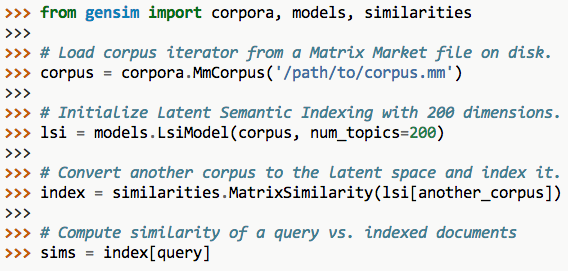
\includegraphics[width=90mm, keepaspectratio]{figures/GensimAbilities.png}
	\caption{Gensim k�pess�gek} 
	\label{fig:GensimAbilities}
\end{figure}

A sz�vegb�ny�szat el�k�sz�t�si �s adatb�ny�szati l�p�seit hivatott megval�s�tani. Er�ss�ge abban rejlik, hogy nem kell k�zzel v�grehajtani a l�p�seket, hanem a weboldalba be�p�lve k�pes a szerveren elv�gezni az �sszes feladatot. 

A gensim seg�ts�g�vel v�gzem el a dokumentum vektor transzform�ci�j�t, a sz�t�r �s a corpus l�trehoz�s�t, a tf-idf elemz�st �s az LSI transzform�ci�t is.

%----------------------------------------------------------------------------
\subsection{Gensim funkci�k}
%----------------------------------------------------------------------------
A gensim a procedur�lis feldolgoz�s jegy�ben a kor�bban ismertetett adat- �s sz�vegb�ny�szati l�p�seket a k�vetkez� funkci�k seg�ts�g�vel val�s�tja meg: 
 
\textbf{Corpus �s Vektort�r kezel�s}: A dokumentumok feldolgoz�sakor String-list�kat haszn�l, hiszen ezeket k�nny� v�gigiter�lni p�ld�ul a stop-szavak kisz�r�s�hez. Automatikusan elv�gzi a szavak tokeniz�ci�j�t (azaz az �sszef�gg� sz�vegb�l a sz�k�z�k ment�n t�rt�n� feldarabol�s�t) �s l�trehozza a sz�t�rat bel�l�k. L�trehozza a sz�gyakoris�g-el�fordul�s vektort. K�pes az eml�tett vektorok �sszess�g�t (a corpus-t) egy�tt kezelni.

\textbf{Corpus, mint m�trix}: a m�trix m�veletek seg�ts�g�vel gyors�tja a feldolgoz�st. A corpus-t a gensim m�r mint m�trixot t�rolja.

\textbf{Matematikai modulok}: a NumPy �s SciPy matematikai f�ggv�nyk�nyvt�rak felhaszn�l�s�val v�gezz�k el a k�l�nb�z� transzform�ci�kat, m�veleteket. 

\textbf{Transzform�ci�k}: k�nnyed�n tudunk bag of words, tf-idf, vagy b�rmilyen, saj�t magunk �ltal defini�lt vektorteret el��ll�tani, egyikb�l a m�sikba transzform�lni.

\textbf{Hasonl�s�gi elemz�s}: k�l�nb�z� vektorok k�z�tti t�vols�g sz�m�t�s�t is elv�gzi, a hasonl�s�gi mutat�k szerint k�nnyed�n kiv�laszthatjuk egy dokumentum t�maszomsz�djait.

%----------------------------------------------------------------------------
\chapter{A \LaTeX-sablon haszn�lata}
%----------------------------------------------------------------------------
Ebben a fejezetben r�viden, implicit m�don bemutatjuk a sablon haszn�lat�nak m�dj�t, ami azt jelenti, hogy sablon haszn�lata ennek a dokumentumnak a forr�sk�dj�t tanulm�nyozva v�lik teljesen vil�goss�. Amennyiben a szoftver-keretrendszer telep�tve van, a sablon alkalmaz�sa �s a dolgozat szerkeszt�se \LaTeX-ben a sablon seg�ts�g�vel tapasztalataink szerint j�val hat�konyabb, mint egy WYSWYG (\emph{What You See is What You Get}) t�pus� sz�vegszerkeszt� eset�n (pl. Microsoft Word, OpenOffice).

%----------------------------------------------------------------------------
\section{C�mk�k �s hivatkoz�sok}
%----------------------------------------------------------------------------
A \LaTeX~dokumentumban c�mk�ket (\verb+\label+) rendelhet�nk �br�khoz, t�bl�zatokhoz, fejezetekhez, list�khoz, k�pletekhez stb. Ezekre a dokumentum b�rmely r�sz�ben hivatkozhatunk, a hivatkoz�sok automatikusan felold�sra ker�lnek.

A sablonban makr�kat defini�ltunk a hivatkoz�sok megk�nny�t�s�hez. Ennek megfelel�en minden �bra (\emph{figure}) c�mk�je \verb+fig:+ kulcssz�val kezd�dik, m�g minden t�bl�zat (\emph{table}), k�plet (\emph{equation}), fejezet (\emph{section}) �s lista (\emph{listing}) rendre a \verb+tab:+, \verb+eq:+, \verb+sect:+ �s \verb+listing:+ kulcssz�val kezd�dik, �s a kulcsszavak ut�n tetsz�legesen v�lasztott c�mke haszn�lhat�. Ha ezt a konvenci�t betartjuk, akkor az el�bbi objektumok sz�m�ra rendre a \verb+\figref+, \verb+\tabref+, \verb+\eqref+, \verb+\sectref+ �s \verb+\listref+ makr�kkal hivatkozhatunk. A makr�k param�tere a c�mke, amelyre hivatkozunk (a kulcssz� n�lk�l). Az �sszes eml�tett hivatkoz�st�pus, bele�rtve az \verb+\url+ kulcssz�val bevezetett web-hivatkoz�sokat is a  \verb+hyperref+\footnote{Seg�ts�g�vel a dokumentumban megjelen� hivatkoz�sok nem csak dinamikuss� v�lnak, de sz�nezhet�k is, b�vebbet err�l a csomag dokument�ci�j�ban tal�lunk. Ez egy�ttal egy p�lda l�bjegyzet �r�s�ra.} csomagnak k�sz�nhet�en akt�vak a legt�bb PDF-n�zeget�ben, r�juk kattintva a dokumentum megfelel� oldal�ra ugrik a PDF-n�z� vagy a megfelel� linket megnyitja az alap�rtelmezett b�ng�sz�vel. A \verb+hyperref+ csomag a kimeneti PDF-dokumentumba k�nyvjelz�ket is k�sz�t a tartalomjegyz�kb�l. Ez egy szint�n akt�v tartalomjegyz�k, amelynek elemeire kattintva a n�zeget� behozza a kiv�lasztott fejezetet.

%----------------------------------------------------------------------------
\section{�br�k �s t�bl�zatok}
%----------------------------------------------------------------------------
A k�peket PDFLaTeX eset�n a vesztes�gmentes PNG, valamint a vesztes�ges JPEG form�tumban �rdemes elmenteni. Az EPS (PostScript) vektorgrafikus k�pform�tum beilleszt�s�t a PDFLatex k�zvetlen�l nem t�mogatja. Ehelyett egy lehet�s�g 200 dpi, vagy ann�l nagyobb felbont�sban raszteriz�lni a k�pet, �s PNG form�tumban elmenteni. Az egyes k�pek m�rete �ltal�ban nem, de sok k�p eset�n a dokumentum �sszm�rete �gy m�r szignifik�ns is lehet. A dokumentumban felhaszn�lt k�pf�jlokat a dokumentum forr�sa mellett �rdemes tartani, archiv�lni, mivel ezek hi�ny�ban a dokumentum nem fordul �jra. Ha lehet, a vektorgrafikus k�peket vektorgrafikus form�tumban is �rdemes elmenteni az �jrafelhaszn�lhat�s�g (az �tszerkeszthet�s�g) �rdek�ben.

Kapcsol�si rajzok legt�bbsz�r kim�solhat�k egy vektorgrafikus programba (pl. CorelDraw) �s onnan nagyobb felbont�ssal raszteriz�lva kimenthat�k PNG form�tumban. Ugyanakkor kiv�l� �br�k k�sz�thet�k Microsoft Visio vagy hasonl� program haszn�lat�val is: Visio-b�l az �br�k k�zvetlen�l PNG-be is menthet�k.

Lehet�s�geink Matlab �br�k eset�n:
\begin{itemize}
	\item K�perny�lop�s (\emph{screenshot}) is elfogadhat� min�s�g� lehet a dokumentumban, de �ltal�ban jobb felbont�st is el lehet �rni m�s m�dszerrel.
	\item A Matlab �br�t a \verb+File/Save As+ opci�val lementhetj�k PNG form�tumban (ugyanaz itt is �rv�nyes, mint kor�bban, ez�rt nem javasoljuk).
	\item A Matlab �br�t az \verb+Edit/Copy figure+ opci�val kim�solhatjuk egy vektorgrafikus programba is �s onnan nagyobb felbont�ssal raszteriz�lva kimenthatj�k PNG form�tumban (nem javasolt).
	\item Javasolt megold�s: az �br�t a \verb+File/Save As+ opci�val EPS \emph{vektorgrafikus} form�tumban elmentj�k, PDF-be konvert�lva beillesztj�k a dolgozatba.
\end{itemize}
Az EPS k�p az \verb+epstopdf+ programmal\footnote{a kor�bban eml�tett \LaTeX-disztrib�ci�kban megtal�lhat�} konvert�lhat� PDF form�tumba. C�lszer� egy batch-f�jlt k�sz�teni az �sszes EPS �bra leford�t�s�ra az al�bbi m�don (ez Windows alatt m�k�dik).
\begin{lstlisting}[frame=single,float=!ht]
@echo off
for %%j in (*.eps) do (
echo converting file "%%j"
epstopdf "%%j"
)
echo done .
\end{lstlisting}

Egy ilyen parancsf�jlt (\verb+convert.cmd+) elhelyezt�k a sablon \verb+figures\eps+ k�nyvt�r�ba, �gy a felhaszn�l�nak csak annyi a dolga, hogy a \verb+figures\eps+ k�nyvt�rba kimenti az EPS form�tum� vektorgrafikus k�pet, majd lefuttatja a \verb+convert.cmd+ parancsf�jlt, ami PDF-be konvert�lja az EPS f�jlt.

Ezek ut�n a PDF-�br�t ugyan�gy lehet a dokumentumba beilleszteni, mint a PNG-t vagy a JPEG-et. A megold�s el�nye, hogy a leford�tott dokumentumban is vektorgrafikusan t�rol�dik az �bra, �gy a m�rete j�val kisebb, mintha raszteriz�ltuk volna beilleszt�s el�tt. Ez a m�dszer minden -- az EPS form�tumot ismer� -- vektorgrafikus program (pl. CorelDraw) eset�n is haszn�lhat�.

A k�pek beilleszt�s�re az \sectref{LatexTools}. fejezetben mutattunk be p�ld�t (\figref{TexnicCenter}~�bra). Az el�z� mondatban egy�ttal az automatikusan felold�d� �brahivatkoz�sra is l�thatunk p�ld�t. T�bb k�pf�jlt is beilleszthet�nk egyetlen �br�ba. Az egyes k�pek k�z�tti horizont�lis �s vertik�lis marg�t metrikusan szab�lyozhatjuk (\figref{HVSpaces}~�bra). Az �br�k elhelyez�s�t sz�mtalan tipogr�fiai szab�ly egyidej� teljes�t�s�vel a ford�t� maga v�gzi, a dokumentum �r�ja csak preferenci�it jelezheti a ford�t� fel� (olykor ez bossz�s�got is okozhat, ilyenkor pl. a k�p m�ret�vel lehet j�tszani).

\begin{figure}[!ht]
\centering
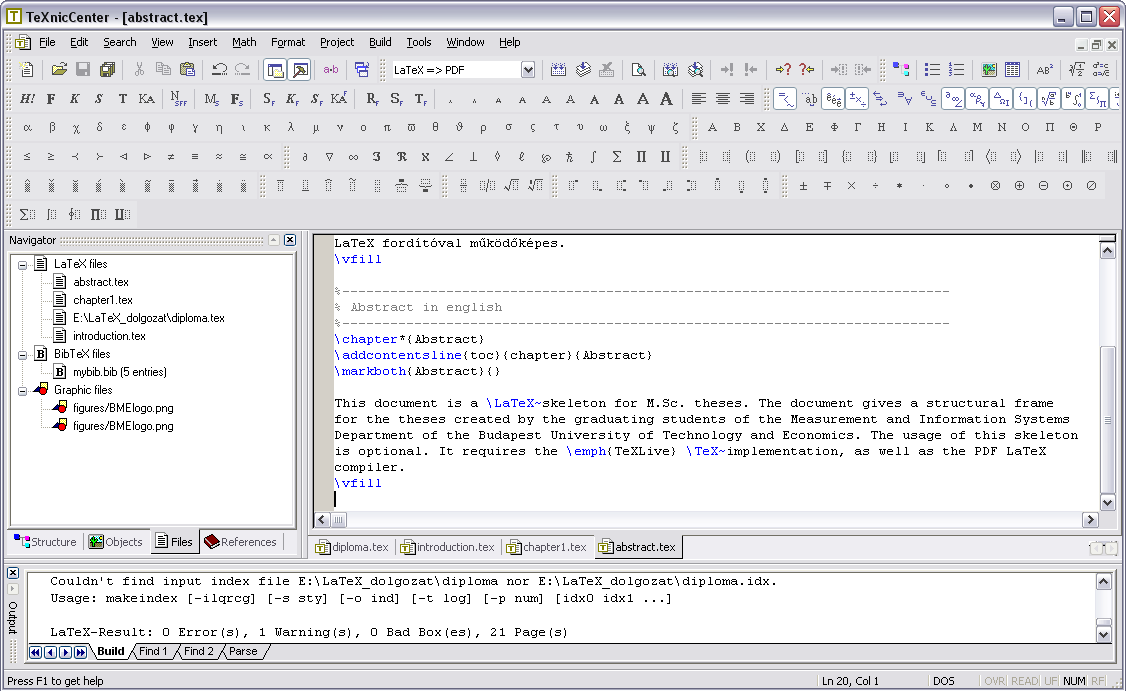
\includegraphics[width=67mm, keepaspectratio]{figures/TeXnicCenter.png}\hspace{1cm}
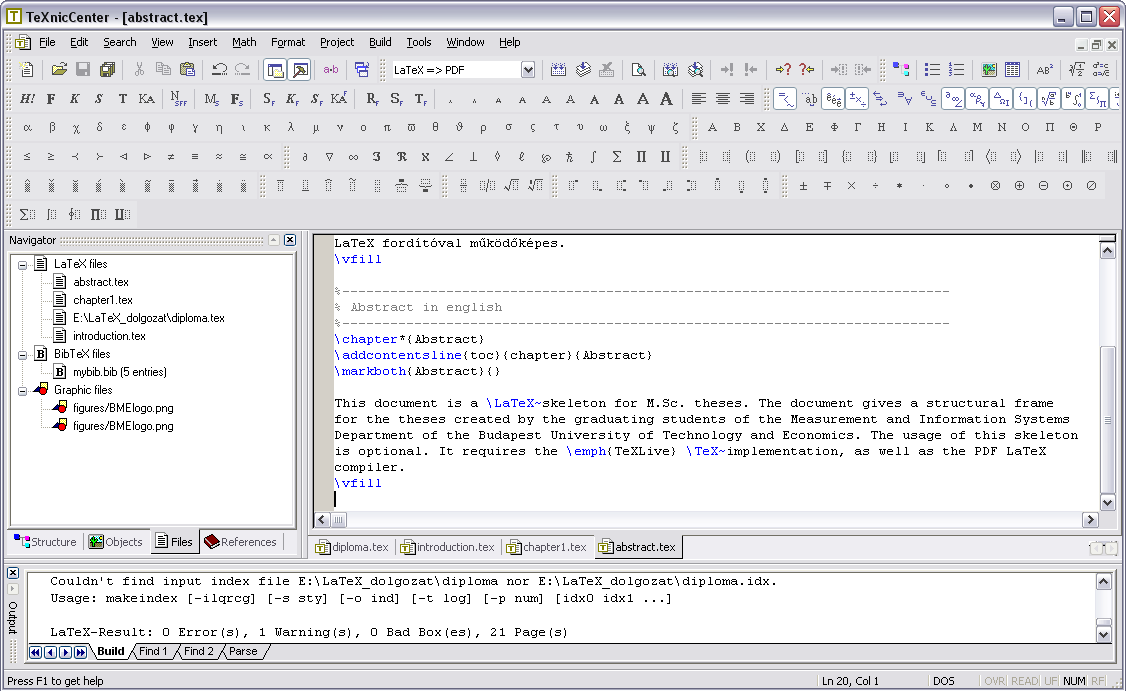
\includegraphics[width=67mm, keepaspectratio]{figures/TeXnicCenter.png}\\\vspace{5mm}
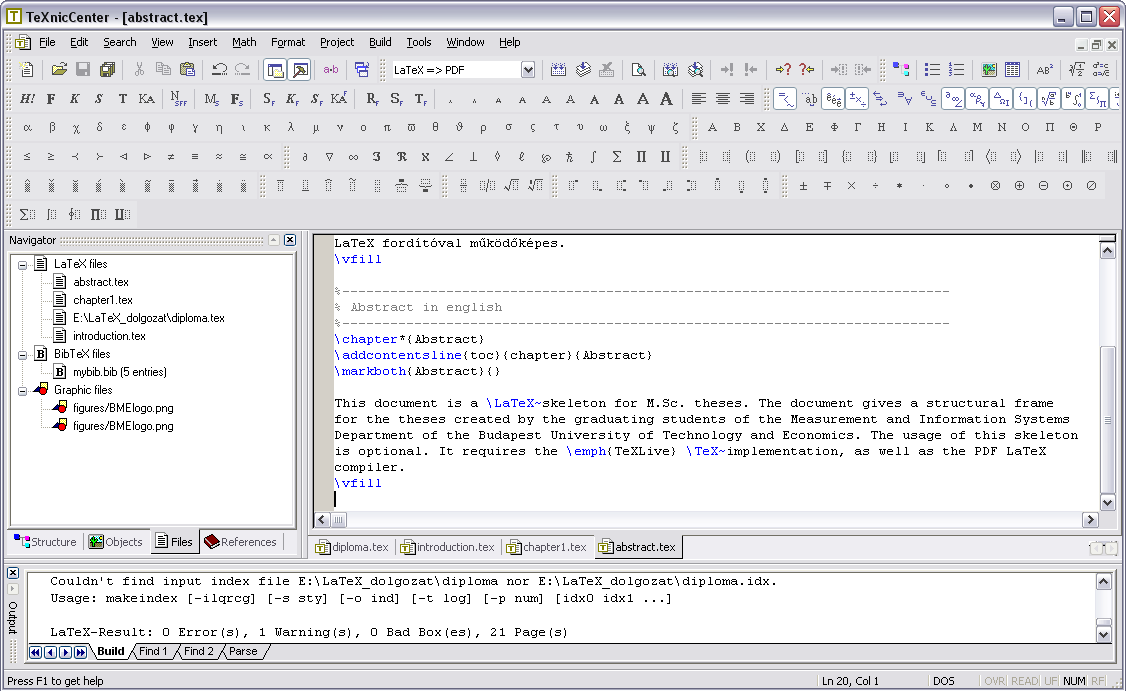
\includegraphics[width=67mm, keepaspectratio]{figures/TeXnicCenter.png}\hspace{1cm}
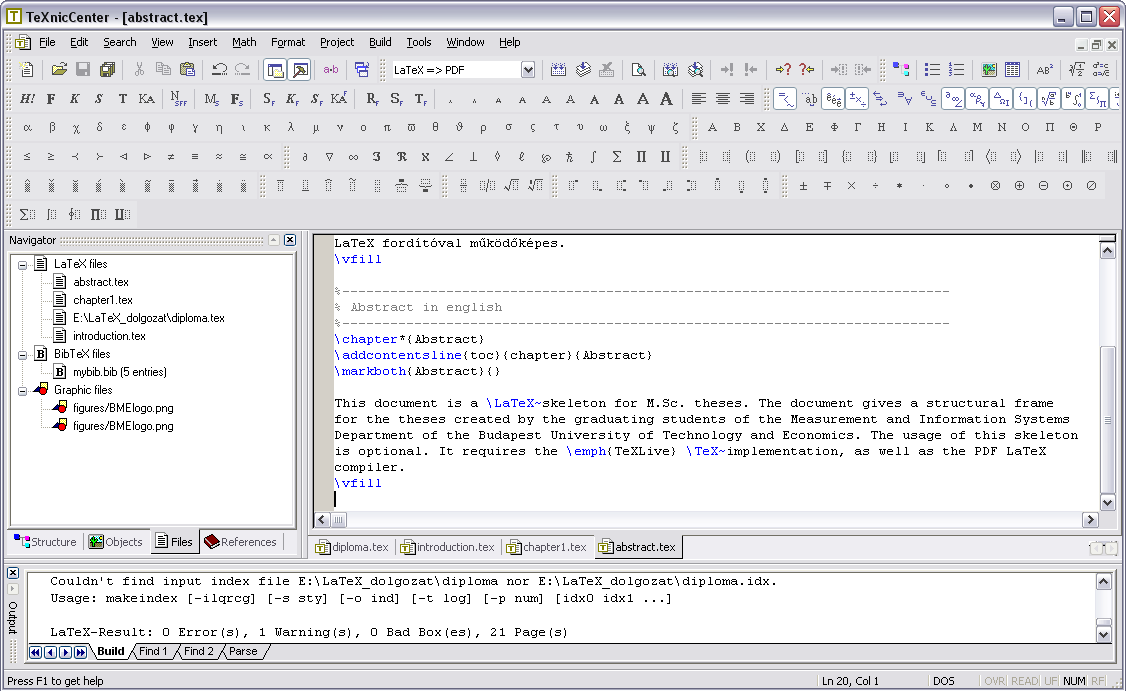
\includegraphics[width=67mm, keepaspectratio]{figures/TeXnicCenter.png}
\caption{T�bb k�pf�jl beilleszt�se eset�n t�rk�z�ket is �rdemes haszn�lni.} 
\label{fig:HVSpaces}
\end{figure}

A t�bl�zatok haszn�lat�ra a \tabref{TabularExample}~t�bl�zat mutat p�ld�t.
A t�bl�zat c�mk�je nem v�letlen�l ker�lt a t�bl�zat f�l�, ez a szokv�nyos.
\begin{table}[ht]
	\footnotesize
	\centering
	\caption{Az �rajel-gener�tor chip �rajel-kimenetei.} \label{tab:SysClocks}
	\begin{tabular}{ | l | c | c |}
	\hline
	�rajel & Frekvencia & C�l pin \\ \hline
	CLKA & 100 MHz & FPGA CLK0\\
	CLKB & 48 MHz  & FPGA CLK1\\
	CLKC & 20 MHz  & Processzor\\
	CLKD & 25 MHz  & Ethernet chip \\
	CLKE & 72 MHz  & FPGA CLK2\\
	XBUF & 20 MHz  & FPGA CLK3\\
	\hline
	\end{tabular}
	\label{tab:TabularExample}
\end{table}


%----------------------------------------------------------------------------
\section{Felsorol�sok �s list�k}
%----------------------------------------------------------------------------
Sz�mozatlan felsorol�sra mutat p�ld�t a jelenlegi bekezd�s:
\begin{itemize}
	\item \emph{els� bajusz:} ide lehetne �rni az els� elem kifej�s�t,
	\item \emph{m�sodik bajusz:} ide lehetne �rni a m�sodik elem kifej�s�t,
	\item \emph{ez meg egy szak�ll:} ide lehetne �rni a harmadik elem kifej�s�t.
\end{itemize}

Sz�mozott felsorol�st is k�sz�thet�nk az al�bbi m�don:
\begin{enumerate}
	\item \emph{els� bajusz:} ide lehetne �rni az els� elem kifej�s�t, �s ez a kifejt�s �gy n�z ki, ha t�bb sorosra sikeredik,
	\item \emph{m�sodik bajusz:} ide lehetne �rni a m�sodik elem kifej�s�t,
	\item \emph{ez meg egy szak�ll:} ide lehetne �rni a harmadik elem kifej�s�t.
\end{enumerate}
A felsorol�sokban sorok v�g�n vessz�, az utols� sor v�g�n pedig pont a szok�sos �r�sjel. Ez al�l kiv�telt k�pezhet, ha az egyes elemek t�bb teljes mondatot tartalmaznak.

List�kban a dolgozat sz�veg�t�l elk�l�n�tend� k�dr�szleteket, programsorokat, pszeudo-k�dokat jelen�thet�nk meg (\listref{Example}~lista). 
\begin{lstlisting}[frame=single,float=!ht,caption=A fenti sz�mozott felsorol�s \LaTeX- forr�sk�dja, label=listing:Example]
\begin{enumerate}
	\item \emph{els� bajusz:} ide lehetne �rni az els� elem kifej�s�t, 
	�s ez a kifejt�s �gy n�z ki, ha t�bb sorosra sikeredik,
	\item \emph{m�sodik bajusz:} ide lehetne �rni a m�sodik elem kifej�s�t,
	\item \emph{ez meg egy szak�ll:} ide lehetne �rni a harmadik elem kifej�s�t.
\end{enumerate}
\end{lstlisting}
A lista keret�t, h�tt�rsz�n�t, eg�sz st�lus�t megv�laszthatjuk. R�ad�sul k�l�nf�le programnyelveket �s a nyelveken bel�l kulcsszavakat is defini�lhatunk, ha sz�ks�ges. Err�l b�vebbet a \verb+listings+ csomag hivatalos le�r�s�ban tal�lhatunk.

%----------------------------------------------------------------------------
\section{K�pletek}
%----------------------------------------------------------------------------
Ha egy formula nem t�ls�gosan hossz�, �s nem akarjuk hivatkozni a sz�vegb�l, mint p�ld�ul a $e^{i\pi}+1=0$ k�plet, \emph{sz�vegk�zi k�pletk�nt} szok�s le�rni. Csak, hogy m�sik p�ld�t is l�ssunk, az $U_i=-d\Phi/dt$ Faraday-t�rv�ny a $\rot E=-\frac{dB}{dt}$ differenci�lis alakban adott Maxwell-egyenlet fel�letre vett integr�lj�b�l vezethet� le. L�that�, hogy a \LaTeX-ford�t� a sork�z�ket betartja, �gy a sz�veg szed�se eszt�tikus marad sz�vegk�zi k�pletek haszn�lata eset�n is.

K�pletek eset�n az �ltal�nos konvenci�, hogy a kisbet�k skal�rt, a kis f�lk�v�r bet�k ($\mathbf{v}$) oszlopvektort -- �s ennek megfelel�en $\mathbf{v}^T$ sorvektort -- a kapit�lis f�lk�v�r bet�k ($\mathbf{V}$) m�trixot jel�lnek. Ha ett�l el szeretn�nk t�rni, akkor az alkalmazni k�v�nt jel�l�sm�dot c�lszer� k�l�n alfejezetben defini�lni. Ennek megfelel�en, amennyiben $\mathbf{y}$ jel�li a m�r�sek vektor�t, $\mathbf{\vartheta}$ a param�terek vektor�t �s $\hat{\mathbf{y}}=\mathbf{X}\vartheta$ a param�terekben line�ris modellt, akkor a \emph{Least-Squares} �rtelemben optim�lis param�terbecsl� $\hat{\mathbf{\vartheta}}_{LS}=(\mathbf{X}^T\mathbf{X})^{-1}\mathbf{X}^T\mathbf{y}$ lesz.

Emellett kiemelt, sorsz�mozott k�pleteket is megadhatunk, enn�l az \verb+equation+ �s a \verb+eqnarray+ k�rnyezetek helyett a korszer�bb \verb+align+ k�rnyezet alkalmaz�s�t javasoljuk (t�bb okb�l, k�l�nf�le probl�m�k elker�l�se v�gett, amelyekre most nem t�r�nk ki). Teh�t
\begin{align}
\dot{\mathbf{x}}&=\mathbf{A}\mathbf{x}+\mathbf{B}\mathbf{u},\\
\mathbf{y}&=\mathbf{C}\mathbf{x},
\end{align}
ahol $\mathbf{x}$ az �llapotvektor, $\mathbf{y}$ a m�r�sek vektora �s $\mathbf{A}$, $\mathbf{B}$ �s $\mathbf{C}$ a rendszert le�r� param�term�trixok. Figyelj�k meg, hogy a k�t egyenletben az egyenl�s�gjelek egym�shoz igaz�tva jelennek meg, mivel a mindkett�t az \& karakter el�zi meg a k�dban. Lehet�s�g van sz�mozatlan kiemelt k�plet haszn�lat�ra is, p�ld�ul
\begin{align}
\dot{\mathbf{x}}&=\mathbf{A}\mathbf{x}+\mathbf{B}\mathbf{u},\nonumber\\
\mathbf{y}&=\mathbf{C}\mathbf{x}\nonumber.
\end{align}
M�trixok fel�r�s�ra az $\mathbf{A}\mathbf{x}=\mathbf{b}$ inhomog�n line�ris egyenlet r�szletes kifejt�s�vel mutatunk p�ld�t:
\begin{align}
\begin{bmatrix}
a_{11} & a_{12} & \dots & a_{1n}\\
a_{21} & a_{22} & \dots & a_{2n}\\
\vdots & \vdots & \ddots & \vdots\\
a_{m1} & a_{m2} & \dots & a_{mn}
\end{bmatrix}
\begin{pmatrix}x_1\\x_2\\\vdots\\x_n\end{pmatrix}=
\begin{pmatrix}b_1\\b_2\\\vdots\\b_m\end{pmatrix}.
\end{align}
A \verb+\frac+ utas�t�s hat�konys�g�t egy �ltal�nos m�sodfok� tag �tviteli f�ggv�ny�n kereszt�l mutatjuk be, azaz
\begin{align}
W(s)=\frac{A}{1+2T\xi s+s^2T^2}.
\end{align}
A matematikai m�d minden szimb�lum�nak �s k�pess�g�nek a bemutat�s�ra term�szetesen itt nincs lehet�s�g, de gyors referenciak�nt hat�konyan haszn�lhat�k a k�vetkez� linkek:\\
\indent\url{http://www.artofproblemsolving.com/LaTeX/AoPS_L_GuideSym.php},\\
\indent\url{http://www.ctan.org/tex-archive/info/symbols/comprehensive/symbols-a4.pdf},\\
\indent\url{ftp://ftp.ams.org/pub/tex/doc/amsmath/short-math-guide.pdf}.\\
Ez pedig itt egy magyar�zat, hogy mi�rt �rdemes \verb+align+ k�rnyezetet haszn�lni:\\
\indent\url{http://texblog.net/latex-archive/maths/eqnarray-align-environment/}.

%----------------------------------------------------------------------------
\section{Irodalmi hivatkoz�sok}\label{sect:HowtoReference}
%----------------------------------------------------------------------------
Egy \LaTeX dokumentumban az irodalmi hivatkoz�sok defin�ci�j�nak k�t m�dja van. Az egyik a \verb+\thebibliograhy+ k�rnyezet haszn�lata a dokumentum v�g�n, az \verb+\end{document}+ lez�r�s el�tt.
\begin{lstlisting}[frame=single,float=!ht]
\begin{thebibliography}{9}

\bibitem{Lamport94} Leslie Lamport, \emph{\LaTeX: A Document Preparation System}. 
Addison Wesley, Massachusetts, 2nd Edition, 1994.

\end{thebibliography}
\end{lstlisting}

Ezek ut�n a dokumentumban a \verb+\cite{Lamport94}+ utas�t�ssal hivatkozhatunk a forr�sra. A fenti megad�s viszonylag k�tetlen, a szerz� maga form�zza az irodalomjegyz�ket. 

Egy sokkal professzion�lisabb m�dszer a BiB\TeX~haszn�lata, ez�rt ez a sablon is ezt t�mogatja. Ebben az esetben egy k�l�n sz�veges adatb�zisban defini�ljuk a forr�smunk�kat, �s egy k�l�n st�lusf�jl hat�rozza meg az irodalomjegyz�k kin�zet�t. Ez, �sszhangban azzal, hogy k�l�n form�tumkonvenci� hat�rozza meg a foly�irat-, a k�nyv-, a konferenciacikk- stb. hivatkoz�sok kin�zet�t az irodalomjegyz�kben (a sablon haszn�lata eset�n ezzel nem is kell foglalkoznia a hallgat�nak, de az eredm�nyt c�lszer� ellen�rizni). A felhaszn�lt hivatkoz�sok adatb�zisa egy \verb+.bib+ kiterjeszt�s� sz�veges f�jl, amelynek szerkezet�t a \listref{Bibtex} k�dr�szlet demonstr�lja. A forr�smunk�k bevitelekor a sor v�gi vessz�k k�l�n figyelmet ig�nyelnek, mert hi�nyuk a BiB\TeX-ford�t� hiba�zenet�t eredm�nyezi. A forr�smunk�kat t�pus szerinti kulcssz� vezeti be (\verb+@book+ k�nyv, \verb+@inproceedings+ konferenciakiadv�nyban megjelent cikk, \verb+@article+ foly�iratban megjelent cikk, \verb+@techreport+ valamelyik egyetem gondoz�s�ban megjelent m�szaki tanulm�ny, \verb+@manual+ m�szaki dokument�ci� eset�n stb.). Nemcsak a megjelen�s st�lusa, de a k�telez�en megadand� mez�k is t�pusr�l-t�pusra v�ltoznak. Egy j�l haszn�lhat� referencia a \url{http://en.wikipedia.org/wiki/BibTeX} oldalon tal�lhat�.
\begin{lstlisting}[frame=single,float=!ht,caption=P�lda sz�veges irodalomjegyz�k-adatb�zisra BiBTeX haszn�lata eset�n., label=listing:Bibtex]
@BOOK{Wettl04,
  author="Ferenc Wettl and Gyula Mayer and P�ter Szab�",
  title="\LaTeX~k�zik�nyv",
  publisher="Panem K�nyvkiad�",
  year=2004
}
@ARTICLE{Candy86,
  author ="James C. Candy",
  title  ="Decimation for Sigma Delta Modulation",
  journal="{IEEE} Trans.\ on Communications",
  volume =34,
  number =1,
  pages  ="72--76",
  month  =jan,
  year   =1986,
}
@INPROCEEDINGS{Lee87,
  author =       "Wai L. Lee and Charles G. Sodini",
  title =        "A Topology for Higher Order Interpolative Coders",
  booktitle =    "Proc.\ of the IEEE International Symposium on 
  Circuits and Systems",
  year =         1987,
  vol =          2,
  month =        may # "~4--7",
  address =      "Philadelphia, PA, USA",
  pages =        "459--462"
}
@PHDTHESIS{KissPhD,
  author =   "Peter Kiss",
  title =    "Adaptive Digital Compensation of Analog Circuit Imperfections 
  for Cascaded Delta-Sigma Analog-to-Digital Converters",
  school =   "Technical University of Timi\c{s}oara, Romania",
  month =    apr,
  year =     2000
}
@MANUAL{Schreier00,
  author = "Richard Schreier",
  title  = "The Delta-Sigma Toolbox v5.2",
  organization = "Oregon State University",
  year   = 2000,
  month  = jan,
  note   ="\newline URL: http://www.mathworks.com/matlabcentral/fileexchange/"
}
@MISC{DipPortal,
	author="Budapesti {M}�szaki �s {G}azdas�gtudom�nyi {E}gyetem 
	{V}illamosm�rn�ki �s {I}nformatikai {K}ar",
  title="{D}iplomaterv port�l (2011 febru�r 26.)",
  howpublished="\url{http://diplomaterv.vik.bme.hu/}",
}}
\end{lstlisting}

A st�lusf�jl egy \verb+.sty+ kiterjeszt�s� f�jl, de ezzel l�nyeg�ben nem kell foglalkozni, mert vannak be�p�tett st�lusok, amelyek j�l haszn�lhat�k. Ez a sablon a BiB\TeX-et haszn�lja, a hozz� tartoz� adatb�zisf�jl a \verb+mybib.bib+ f�jl. Megfigyelhet�, hogy az irodalomjegyz�ket a dokumentum v�g�re (a \verb+\end{document}+ utas�t�s el�) beillesztett \verb+\bibliography{mybib}+ utas�t�ssal hozhatjuk l�tre, a st�lus�t pedig ugyanitt a  \verb+\bibliographystyle{plain}+ utas�t�ssal adhatjuk meg. Ebben az esetben a \verb+plain+ el�re defini�lt st�lust haszn�ljuk (a sablonban is ezt �ll�tottuk be). A \verb+plain+ st�luson k�v�l term�szetesen sz�mtalan m�s el�re defini�lt st�lus is l�tezik. Mivel a \verb+.bib+ adatb�zisban ezeket megadtuk, a BiB\TeX-ford�t� is meg tudja k�l�nb�ztetni a szerz�t a c�mt�l �s a kiad�t�l, �s ez alapj�n automatikusan gener�l�dik az irodalomjegyz�k a st�lusf�jl �ltal meghat�rozott st�lusban.

Az egyes forr�smunk�kra a sz�vegb�l tov�bbra is a \verb+\cite+ paranccsal tudunk hivatkozni, �gy a \listref{Bibtex} k�dr�szlet eset�n a hivatkoz�sok rendre \verb+\cite{Wettl04}+, \verb+\cite{Candy86}+, \verb+\cite{Lee87}+, \verb+\cite{KissPhD}+, \verb+\cite{Schreirer00}+ �s \verb+\cite{DipPortal}+. Az irodalomjegyz�kben alap�rtelmez�sben csak azok a forr�smunk�k jelennek meg, amelyekre tal�lhat� hivatkoz�s a sz�vegben, �s ez �gy alapvet�en helyes is, hiszen olyan forr�smunk�kat nem illik az irodalomjegyz�kbe �rni, amelyekre nincs hivatkoz�s.

Mivel a ford�t�si folyamat sor�n t�bb l�p�sben old�dnak fel a szimb�lumok, ez�rt gyakran t�bbsz�r (TeXLive �s TeXnicCenter eset�n 2-3-szor) is le kell ford�tani a dokumentumot. Ilyenkor ez els� 1-2 ford�t�s esetleg szimb�lum-felold�sra vonatkoz� figyelmeztet� �zenettel z�rul. Ha hiba�zenettel z�rul b�rmelyik ford�t�s, akkor nincs �rtelme megism�telni, hanem a hib�t kell megkeresni. A \verb+.bib+ f�jl megv�ltoztat�skor sokszor nincs hat�sa a v�ltoztat�snak azonnal, mivel nem mindig fut �jra a BibTeX ford�t�. Ez�rt c�lszer� a v�ltoztat�s ut�n azt manu�lisan is lefuttatni (TeXnicCenter eset�n \verb+Build/BibTeX+).

Hogy a sz�vegbe �gyazott hivatkoz�sok kin�zet�t demonstr�ljuk, itt most sorban meghivatkozzuk a \cite{Wettl04}, \cite{Candy86}, \cite{Lee87}, \cite{KissPhD} �s az \cite{Schreier00} forr�smunk�t, valamint az \cite{DipPortal} weboldalt.

Megjegyzend�, hogy az �kezetes magyar bet�ket is tartalmaz� \verb+.bib+ f�jl az \verb+inputenc+ csomaggal bet�lt�tt \verb+latin2+ bet�k�szlet miatt ford�that�. Ugyanez a \verb+.bib+ f�jl hiba�zenettel fordul egy olyan dokumentumban, ami nem tartalmazza a \verb+\usepackage[latin2]{inputenc}+ sort. Speci�lis ig�ny eset�n az irodalmi adatb�zis �ltal�nosabb �rv�ny�v� tehet�, ha az �kezetes bet�ket speci�lis latex karakterekkel helyettes�tj�k a \verb+.bib+ f�jlban, pl. � helyett \verb+\'{a}+-t vagy � helyett \verb+\H{o}+-t �runk. 

Oldalt�r�s k�vetkezik (ld. forr�s).
\newpage

%----------------------------------------------------------------------------
\section{A dolgozat szerkezete �s a forr�sf�jlok}
%----------------------------------------------------------------------------
A diplomatervsablon (a kari ir�nyelvek szerint) az al�bbi f� fejezetekb�l �ll:
\begin{enumerate}
	\item 1 oldalas \emph{t�j�koztat�} a szakdolgozat/diplomaterv szerkezet�r�l (\verb+guideline.tex+), ami a v�gs� dolgozatb�l t�rlend�,
	\item \emph{feladatki�r�s} (\verb+project.tex+), a dolgozat nyomtatott verz�j�ban ennek a hely�re ker�l a tansz�k �ltal kiadott, a tansz�kvezet� �ltal al��rt feladatki�r�s, a dolgozat elektronikus verzi�j�ba pedig a feladatki�r�s egy�ltal�n ne ker�lj�n bele, azt k�l�n t�lti fel a tansz�k a diplomaterv-honlapra,
	\item \emph{c�moldal} (\verb+titlepage.tex+),
	\item \emph{tartalomjegyz�k} (\verb+diploma.tex+),
	\item a diplomatervez� \emph{nyilatkozat}a az �n�ll� munk�r�l (\verb+declaration.tex+),
	\item 1-2 oldalas tartalmi \emph{�sszefoglal�} magyarul �s angolul, illetve elk�sz�thet� m�g tov�bbi nyelveken is (\verb+abstract.tex+),
	\item \emph{bevezet�s}: a feladat �rtelmez�se, a tervez�s c�lja, a feladat indokolts�ga, a diplomaterv fel�p�t�s�nek r�vid �sszefoglal�sa (\verb+introduction.tex+),
	\item sorsz�mmal ell�tott \emph{fejezetek}: a feladatki�r�s pontos�t�sa �s r�szletes elemz�se, el�zm�nyek (irodalomkutat�s, hasonl� alkot�sok), az ezekb�l levonhat� k�vetkeztet�sek, a tervez�s r�szletes le�r�sa, a d�nt�si lehet�s�gek �rt�kel�se �s a v�lasztott megold�sok indokl�sa, a megtervezett m�szaki alkot�s �rt�kel�se, kritikai elemz�se, tov�bbfejleszt�si lehet�s�gek (\verb+chapter{1,2..n}.tex+),
	\item esetleges \emph{k�sz�netnyilv�n�t�s}ok (\verb+acknowledgement.tex+),
	\item r�szletes �s pontos \emph{irodalomjegyz�k} (ez a sablon eset�ben automatikusan gener�l�dik a \verb+diploma.tex+ f�jlban elhelyezett \verb+\bibliography+ utas�t�s hat�s�ra, a \sectref{HowtoReference}. fejezetben le�rtak szerint),
	\item \emph{f�ggel�kek} (\verb+appendices.tex+).
\end{enumerate}

A sablonban a fejezetek a \verb+diploma.tex+ f�jlba vannak beillesztve \verb+\include+ utas�t�sok seg�ts�g�vel. Lehet�s�g van arra, hogy csak az �ppen szerkeszt�s alatt �ll� \verb+.tex+ f�jlt ford�tsuk le, ezzel ler�vid�tve a ford�t�si folyamatot. Ezt a lehet�s�get az al�bbi k�dr�szlet biztos�tja a \verb+diploma.tex+ f�jlban.
\begin{lstlisting}[frame=single,float=!ht]
\includeonly{
	guideline,%
	project,%
	titlepage,%
	declaration,%
	abstract,%
	introduction,%
	chapter1,%
	chapter2,%
	chapter3,%
	acknowledgement,%
	appendices,%
}
\end{lstlisting}

Ha az al�bbi k�dr�szletben az egyes sorokat a \verb+%+ szimb�lummal kikommentezz�k, akkor a megfelel� \verb+.tex+ f�jl nem fordul le. Az oldalsz�mok �s a tartalomjegy�k term�szetesen csak akkor billennek helyre, ha a teljes dokumentumot leford�tjuk.

%----------------------------------------------------------------------------
\newpage
\section{Alapadatok megad�sa}
%----------------------------------------------------------------------------
A diplomaterv alapadatait (c�m, szerz�, konzulens, konzulens titulusa) a \verb+diploma.tex+ f�jlban lehet megadni az al�bbi k�dr�szlet m�dos�t�s�val.
\begin{lstlisting}[frame=single,float=!ht]
\newcommand{\vikszerzo}{B�dis-Szomor� Andr�s}
\newcommand{\vikkonzulens}{dr.~Konzulens Elem�r}
\newcommand{\vikcim}{Elektronikus terel�k}
\newcommand{\viktanszek}{M�r�stechnika �s Inform�ci�s Rendszerek Tansz�k}
\newcommand{\vikdoktipus}{Diplomaterv}
\newcommand{\vikdepartmentr}{B�dis-Szomor� Andr�s}
\end{lstlisting}

%----------------------------------------------------------------------------
\section{�j fejezet �r�sa}
%----------------------------------------------------------------------------
A f�fejezetek k�l�n \verb+chapter{1..n}.tex+ f�jlban foglalnak helyet. A sablonhoz 3 fejezet k�sz�lt. Tov�bbi f�fejezeteket �gy hozhatunk l�tre, ha �j \verb+chapter{i}.tex+ f�jlt k�sz�t�nk a fejezet sz�m�ra, �s a \verb+diploma.tex+ f�jlban, a \verb+\include+ �s \verb+\includeonly+ utas�t�sok argumentum�ba felvessz�k az �j \verb+.tex+ f�jl nev�t.






%----------------------------------------------------------------------------
\chapter{A mobilapplik�ci� fejleszt�se �s tesztel�se}
%----------------------------------------------------------------------------
A k�vetkez�kben megvizsg�lom a Xamarin keretrendszer fejleszt�si lehet�s�geit.
Ezut�n kit�rek a fejleszt�s sor�n haszn�lt f�bb programoz�si paradigm�kra, majd ismertetem az alkalmaz�slogika strukt�r�j�t, �s az annak implement�l�sa sor�n felmer�lt kih�v�sokat.
Bemutatom a felhaszn�l�i fel�let k�sz�t�sekor haszn�lt Xamarin.Forms k�nyvt�r l�nyegesebb elemeit, valamint azon hib�ikat, amikkel a fejleszt�s sor�n tal�lkoztam.
V�g�l kit�rek arra, milyen m�dokon teszteltem az applik�ci�t az elk�sz�t�se sor�n.

%----------------------------------------------------------------------------
\section{A Xamarin multi-platform fejleszt�si lehet�s�gei}\label{sect:XamarinMultiplatformOptions}
%----------------------------------------------------------------------------
A multi-platform k�d elk�sz�t�s�re a keretrendszer k�t k�l�nb�z� megk�zel�t�st k�n�l: a megosztott projekteket (shared project) \cite{SharedProjOverview} �s a hordozhat� oszt�lyk�nyvt�rakat (portable class library, PCL) \cite{PCLOverview}.

Megosztott projekt haszn�latakor a k�z�s funkci�k mellett a platformspecifikus k�dr�szletek is ugyanabban a forr�sf�jlban kapnak helyet.
A \Csharp~ford�t� preprocesszora sz�m�ra\linebreak\textit{\texttt{\#}if PLATFORM ... \texttt{\#}endif} utas�t�sokkal jelezz�k, melyik c�l-oper�ci�srendszeren milyen k�dot kell futtatnia.
Az �gy k�r�lvett k�dr�szben haszn�lhatjuk az adott platform specifikus k�nyvt�rait is.
Adott platformra ford�t�skor csak az ahhoz tartoz� k�d ker�l be�p�t�sre a v�gleges alkalmaz�scsomagba (\figref{SharedProjFigure} �bra). Ennek a megk�zel�t�snek h�tr�nya, hogy a forr�sf�jl nehezen olvashat�v� v�lhat.

Hordozhat� oszt�lyk�nyvt�r eset�n a k�z�s k�d egy k�l�n DLL-ben\footnote{Dynamic Link Library, dinamikus csatol�s� k�nyvt�r: olyan alkalmaz�s-seg�df�jl, ami t�bbek k�z�tt elj�r�sokat, kompatibilit�st seg�t� eszk�z�ket vagy �gynevezett "er�forr�sokat" (pl. k�peket, hangokat, lokaliz�lt sztringeket) t�rolhat.} kap helyet. Ekkor a megosztott k�dban nem haszn�lhatunk egyedi platformk�nyvt�rakat, hanem interf�szeket defini�lunk a platformspecifikus funkci�k el�r�s�re, amiket a c�l-oper�ci�srendszerek saj�t projektjeiben val�s�tunk meg (\figref{PCLFigure} �bra).
\newpage
\begin{figure}[!ht]
	\centering
	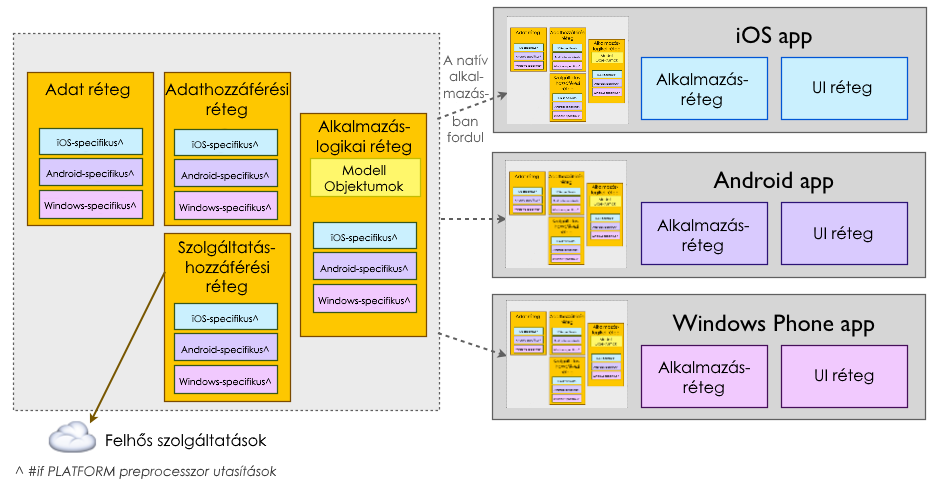
\includegraphics[width=150mm, keepaspectratio]{figures/SharedAssetProject.png}
	\caption{Megosztott projektet haszn�l� alkalmaz�s strukt�r�ja \cite{XamarinCodeSharing}}
	\label{fig:SharedProjFigure}
\end{figure}
\begin{figure}[!hb]
	\centering
	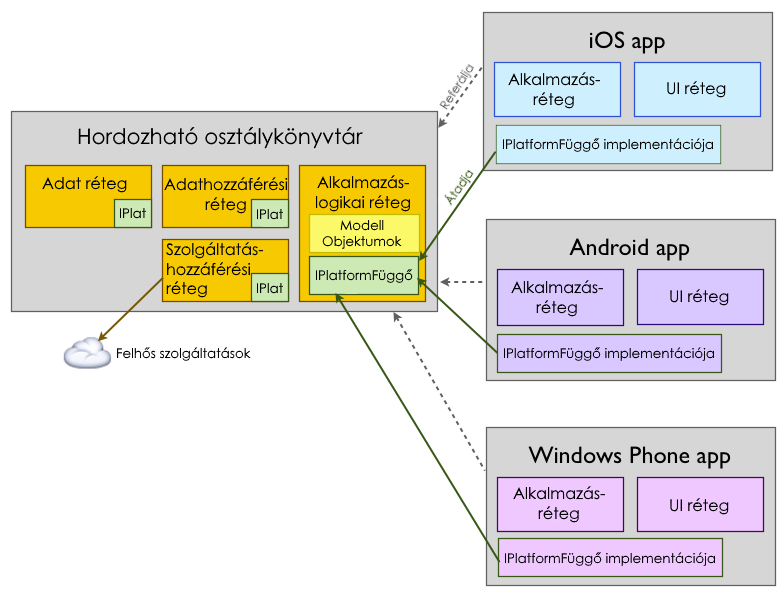
\includegraphics[width=150mm, keepaspectratio]{figures/PCLProject.png}
	\caption{Hordozhat� oszt�lyk�nyvt�rat haszn�l� alkalmaz�s strukt�r�ja \cite{XamarinCodeSharing}}
	\label{fig:PCLFigure}
\end{figure}
\FloatBarrier

A k�z�s k�dban a Xamarin \textit{DependencyService} oszt�ly�nak haszn�lat�val h�vhatjuk meg az oper�ci�srendszer-specifikus f�ggv�nyeket.
Az al�bbi k�dr�szlet egy SQLite adatb�zis megnyit�s�t mutatja az \textit{ISQLite} interf�sz haszn�lat�val:
\begin{lstlisting}[frame=single]
var SQLiteDb = DependencyService.Get<ISQLite>().GetConnection();
\end{lstlisting}

A \textit{Device} oszt�ly ny�jt funkci�kat a programot futtat� eszk�zr�l inform�ci� szerz�s�re, mint p�ld�ul a platform (Android, iOS vagy Windows Phone), az idi�ma (asztali sz�m�t�g�p, telefon vagy tablet) vagy a neves�tett bet�m�retekhez (micro, kicsi, k�zepes, nagy, alap�rtelmezett) tartoz� sz�mszer�s�tett bet�m�ret.
%----------------------------------------------------------------------------
\section{A fejleszt�s sor�n haszn�lt f�bb programoz�si paradigm�k}
%----------------------------------------------------------------------------
%----------------------------------------------------------------------------
\subsection{Az MVVM}\label{sect:MVVM}
%----------------------------------------------------------------------------
Az MVVM egy szoftverarchitekt�ra-tervez�si minta, felold�sa "Model-View-View Model".
Ez a tervez�si minta az MVC (Model-View-Control) minta egy m�dos�tott v�ltozata, amit a Microsoft fejleszt�i a .NET keretrendszer grafikus rendszer�nek (WPF\footnote{A Windows Presentation Foundation egy egys�ges�tett programoz�si modell grafikus alkalmaz�sok k�sz�t�s�re \CsharpDotNet-ben.}) figyelembe v�tel�vel k�sz�tettek az esem�nyalap� felhaszn�l�i fel�let fejleszt�s�nek megk�nny�t�s�re \cite{MicrosoftMVVM}.

A \textit{View} komponens hat�rozza meg a grafikus fel�let strukt�r�j�t, kioszt�s�t �s megjelen�s�t. �zleti logik�t nem tartalmaz, csak a felhaszn�l�i interakci�k (p�ld�ul kattint�s) �rtelmez�se t�rt�nik, majd az esem�nyt k�zli a View Modellel.

A \textit{Model} feladata az adatok reprezent�l�sa, valamint a valid�ci�s- �s �zleti logika megval�s�t�sa. Itt t�rt�nik a kommunik�ci� az alkalmaz�son k�v�li komponensekkel is, p�ld�ul az adatok szinkroniz�l�sa egy t�voli szerverrel.

A \textit{View Model} az �sszek�t� kapocs a Model �s a View k�z�tt. Feladata, hogy a Model �ltal ny�jtott adatokat a View sz�m�ra alkalmas form�ra hozza, illetve a felhaszn�l�i interakci�k hat�s�t �rv�nyes�tse a Modelben. Ezek mellett a View �llapotg�pek�nt is szolg�l, p�ld�ul hosszan tart� m�veletek eset�n utas�thatja a View-t, hogy egy t�lt�k�perny�t jelen�tsen meg.

%----------------------------------------------------------------------------
\subsection{\Csharp~grafikus elemek le�r�sa XAML-ben, adatk�t�s}\label{sect:XamlDataBinding}
%----------------------------------------------------------------------------
A \Csharp-ban �rt grafikus fel�letek strukt�r�j�nak �tl�that�s�g�ra a Microsoft kifejlesztette a XAML-t\footnote{Extensible Application Markup Language, azaz b�v�thet� alkalmaz�sle�r� nyelv.}, ami egy olyan, XML alap� le�r� nyelv, ami az objektumok inicializ�l�s�n �s tagv�lt�z�inak be�ll�t�s�n k�v�l k�nnyen l�that�v� teszi az objektumok k�z�tti hierarchi�t \cite{MicrosoftXAML}.
Lehet�s�g van a be�p�tett t�pusokon t�l tov�bbi t�pusokkal �s b�v�tm�nyekkel kieg�sz�teni az alkalmaz�sunk ig�nyeinek megfelel�en, ak�rcsak a szokv�nyos \Csharp~k�dot.

Egy XAML n�zetle�r� k�t r�szb�l �ll: mag�b�l a le�r�sb�l �s a hozz� tartoz� m�g�ttes k�db�l (Code-Behind).
A m�g�ttes k�db�l el�rhet�ek a XAML le�r�sban deklar�lt objektumok, �s ford�tva, ezzel meghagyva a fejleszt� szabads�g�t, hogy a k�l�nb�z� tulajdons�gok be�ll�t�s�t melyik nyelv haszn�lat�val v�gzi el.
A m�g�ttes k�d feladata az esem�nykezel�k megval�s�t�sa, viszont min�l kevesebb alkalmaz�slogika ker�lj�n ide.

A View Model �ltal megjelen�t�sre alkalmas (vagy ahhoz nagyon k�zeli) form�ra hozott adatokat a grafikus elemekhez rendelj�k, �gynevezett adatk�t�st (data binding) v�gz�nk.
A k�t�s t�pusa Xamarinban lehet egyir�ny� az adatt�l a megjelen�tett elem ir�ny�ba, vagy vissza, illetve k�tir�ny�, ekkor az adat friss�lhet a View Model �s a View ir�ny�b�l is.
Ha a View-beli elem adatforr�sa nem a View-t megval�s�t� oszt�ly tagv�ltoz�ja, akkor Xamarinban az elem \textit{BindingContext} (k�t�si kontextus) tulajdons�g�nak �rt�k�l kell adni azt az objektumot, amiben a k�t�sre sz�nt adat tal�lhat�.
A k�t�si kontextus automatikusan �r�kl�dik, azaz ha a View-t implement�l� oszt�ly BindingContextj�nek adjuk �rt�k�l (tipikusan) a View Modelt, akkor az �sszes benne elhelyezett elem is ugyanazt a k�t�si kontextust kapja, kiv�ve, ha fel�ldefini�ljuk azt.
Ezut�n az adatk�t�sn�l m�r csak a k�t�sikontextus-oszt�ly tagjaira hivatkozunk, amiknek publikus l�that�s�g�nak kell lenni�k.

Ahhoz, hogy a k�t�tt adat friss�t�s�r�l a View �rtes�t�st kapjon, �s friss�tse\linebreak a megjelen�tett elemet, a View Modelnek implement�lnia kell a\linebreak\textit{System.ComponentModel.INotifyPropertyChanged} interf�szt, valamint a k�t�tt adat v�ltoz�sakor meg kell h�vnia saj�t \textit{OnPropertyChanged} implement�ci�j�t.
A f�ggel�k \sectref{SearchExample} pontj�nak k�dr�szletei a mobilapp bar�tkeres�s funkci�j�n kereszt�l szeml�ltetik az adatk�t�st.
Mivel a keres�s�v egy beviteli mez�, ez�rt k�t�se a \textit{SearchFilter} taggal automatikusan k�tir�ny�, �gy a megfelel� \textit{set} elj�r�s haszn�lat�val k�nyelmi funkci�k�nt m�r a keres�sz� megad�sa alatt, minden karakter bevitele ut�n lefut egy sz�r�s a bar�tlist�ra.

%----------------------------------------------------------------------------
\subsection{Aszinkron mechanizmusok}\label{sect:AsyncMechanisms}
%----------------------------------------------------------------------------
A grafikus fel�lettel rendelkez� alkalmaz�sokn�l kiemelked�en fontos, hogy a f� programsz�lon, ami a felhaszn�l�i interf�sz (angolul user interface, UI) megjelen�t�s��rt is felel, a lehet� legkevesebb feladatot futtassuk.
Ezzel biztos�tjuk a fel�let reszponzivit�s�t, azaz az anim�ci�k folyamatoss�g�t �s a felhaszn�l�i input feldolgoz�s�nak gyors megkezd�s�t.

A .NET keretrendszer a 4-es verzi�t�l kezdve rendelkezik egy feladat-p�rhuzamos�t�si k�nyvt�rral (Task Parallel Library, TPL), ami a kor�bban is l�tez� p�rhuzamos�t�si mechanizmusokat egy er�forr�s-hat�konyabb, jobban sk�l�z�d� �s nagyobb kontrollt ny�jt� keretbe fogja �ssze.
Ennek alapegys�ge a feladat (Task oszt�ly), amin t�bbek k�z�tt a szok�sos sz�lkezel�si m�veleteket is v�grehajthatjuk (p�ld�ul ind�t�s, v�rakoz�s, megszak�t�s, a visszat�r�si �rt�k �s kil�p�si k�d lek�rdez�se).

Az egy�rtelm�en id�ig�nyes m�veleteket - p�ld�ul f�jl- �s adatb�zis-m�veletek, kommunik�ci� m�s folyamatokkal �s szolg�ltat�sokkal vagy internetes lek�rdez�sek - mindenk�pp �rdemes h�tt�rsz�lakon futtatni.
Ha a k�zi tesztel�s sor�n azt tapasztaljuk, hogy egy m�velet �rezhet� ideig blokkolja a f� sz�lat, azt is futtathatjuk taszkk�nt.
Kritikus azonban, hogy az adatk�t�tt v�ltoz�k �rt�km�dos�t�s�t mindenk�ppen a f� sz�lban v�gezz�k, mert az adatk�t�s nem sz�lbiztos mechanizmus, �s csak ezzel biztos�that� az �j adatok megjelen�se a fel�leten (l�sd a \sectref{ElementPlacement} pont ObservableCollection haszn�lat�r�l sz�l� r�sz�t).
A f� sz�l h�v�s�t Xamarinban a \textit{Device.BeginInvokeOnMainThread()} f�ggv�nnyel tehetj�k meg, azonban erre a taszkra nem lehet v�rakozni, ez�rt c�lszer� a m�veleteket �gy �temezni, hogy a k�t�sek friss�t�se legyen az utols�. Aj�nlatos tov�bb�, hogy a f� sz�lban logikai m�veletet m�r ne, hanem csak az �rt�kad�st v�gezz�k, ezzel is r�vid�tve annak blokkol�si idej�t.

%----------------------------------------------------------------------------
\section{Az alkalmaz�slogika}
%----------------------------------------------------------------------------
Az alkalmaz�s elk�sz�t�s�hez a PCL megk�zel�t�st v�lasztottam, mert sz�momra az interf�szek haszn�lata tiszt�bb �s �tl�that�bb, mint az egy forr�sf�jlban preprocesszor-utas�t�sokkal tagolt r�szek.

Az alkalmaz�s felhaszn�l�ifel�let-r�teg�nek fejleszt�si lehet�s�geit a \sectref{XamarinResearch} pontban ismertettem.
A platformonk�nt egyedi, ottani diz�jn-ir�nyelveknek teljesen megfelel� felhaszn�l�i fel�letek elk�sz�t�s�t a szakdolgozat keretein t�lmutat� feladatnak tekintett�k konzulensemmel.
A Xamarin.Forms multi-platform fel�letprogramoz�si k�nyvt�r haszn�lata mellett d�nt�tt�nk, ami egys�gesebb kin�zetet ny�jt, �s a hordozhat� oszt�lyk�nyvt�r DLL-ben foglal helyet.

A \figref{AppStructure} �br�n l�that� az alkalmaz�s strukt�r�ja, amit az MVVM tervez�si minta (\sectref{MVVM}  pont) figyelembe v�tel�vel alkottam meg.
A k�vetkez�kben ismertetem az alkalmaz�slogika egyes r�szeinek m�k�d�s�t, a felhaszn�lt k�nyvt�rakat, �s a felmer�lt kih�v�sokat a megval�s�t�s sor�n.
\begin{figure}[!h]
	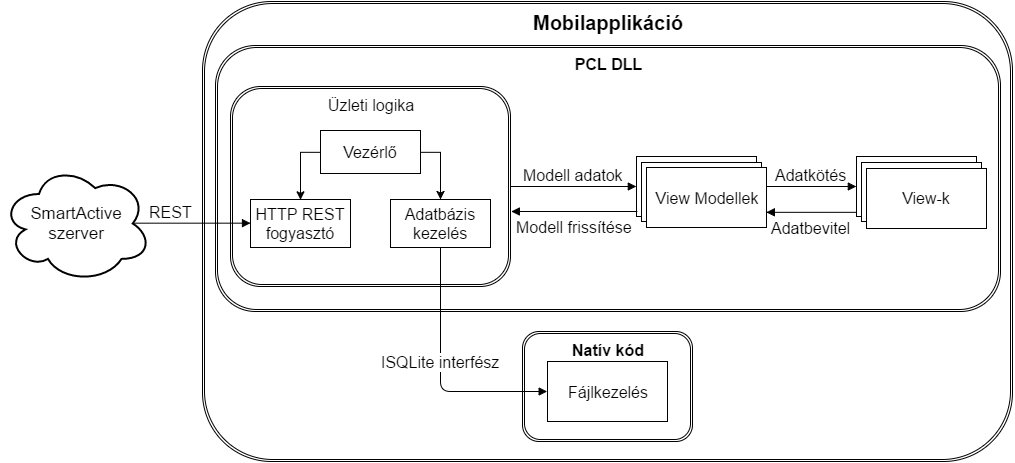
\includegraphics[width=150mm, keepaspectratio]{figures/AppStructure.png}
	\caption{A mobilalkalmaz�s strukt�r�ja}
	\label{fig:AppStructure}
\end{figure}

%----------------------------------------------------------------------------
\subsection{Kommunik�ci� a webszerverrel}
%----------------------------------------------------------------------------
A t�voli szerverrel t�rt�n� �zenetv�lt�shoz HTTP REST\footnote{A Representational State Transfer architekt�r�ban a HTTP webprotokoll URI (Uniform Resource Identifier, egy r�vid karaktersorozat, amelyet egy webes er�forr�s azonos�t�s�ra haszn�lunk, pl. egy honlapc�m) elem�t kihaszn�lva lehet kommunik�lni. Megfelel�en fel�p�tett URI-k haszn�lat�val p�ld�ul a GET �zenet lek�rdez�sre, a POST adatk�ld�sre haszn�lhat�.} �zeneteket haszn�l az alkalmaz�s.
A szerver a szinkroniz�land� adatokat JSON\footnote{A JavaScript Object Notation egy egyszer�en fel�p�tett adatcser�re haszn�lhat� form�tum. Alapegys�ge az objektum, ami egy kulcs-�rt�k p�rb�l �ll. A kulcs mindig egy sztring. Az �rt�k lehet objektum, �rt�keket tartalmaz� t�mb, sztring, sz�m, igaz-hamis �rt�k vagy nullelem \cite{JsonOrg}.} form�tumban k�ldi �t.
Ennek feldolgoz�s�ra a .NET keretrendszer ny�jt egy k�nyvt�rat, de �n a t�bb lehet�s�get k�n�l� Newtonsoft Json.NET-et \cite{NewtonSoftJSON} v�lasztottam.
Ebben ugyanis ha rendelkez�nk egy \Csharp~oszt�llyal, aminek a strukt�r�ja �s tagv�ltoz�nevei megegyeznek a JSON strukt�r�j�val �s kulcssztringjeivel, akkor a rendszer k�pes azonnal deszerializ�lni azt.
A kulcssztring - tagv�ltoz�n�v k�l�nbs�gek feloldhat�k a tagv�ltoz�k megfelel� attrib�tumokkal t�rt�n� ell�t�s�val.

%----------------------------------------------------------------------------
\subsection{Az adatok perziszt�l�sa}
%----------------------------------------------------------------------------
A szinkroniz�lt adatok helyi t�rol�s�t el�sz�r a .NET keretrendszer szerializ�l�si elj�r�saival akartam megval�s�tani, azonban kider�lt, hogy erre hordozhat� oszt�lyk�nyvt�rban nincs lehet�s�g.
Megold�sk�nt egy SQLite adatb�zis l�trehoz�s�t v�lasztottam.

Az SQLite egy egyszer� fel�p�t�s�, szerver-kliens kialak�t�st nem ig�nyl�, kev�s k�ls� f�gg�s�ggel rendelkez�, ak�r el�zetes konfigur�l�s n�lk�l is haszn�lhat� tranzakcion�lis SQL adatb�zismotor \cite{SQLite}.
A teljes adatb�zist egy f�jl t�rolja, ami tartalmazza a s�m�t, a k�nyszereket �s a rekordokat is.
Ez kiv�l�an alkalmass� teszi be�gyazott �s mobileszk�z�kben t�rt�n� haszn�latra.
Tov�bbi �rv a v�laszt�s mellett, hogy az Android �s iOS oper�ci�s rendszerekben integr�lva van az SQLite adatb�zismotor, �gy azt csak a Microsoft mobil oper�ci�s rendszereihez kell k�l�n refer�lni (beszerz�s�ket l�sd a \sectref{CompileSettings} pontban).

T�bbf�le NuGet csomag k�n�l programk�nyvt�rat SQLite adatb�zisok .NET-ben t�rt�n� multi-platform menedzsel�s�hez.
El�sz�r a kapcsol�d� Xamarin �tmutat�ban \cite{XamarinDbGuide} haszn�lt \textit{SQLite-net PCL} \cite{SQLite-netKrueger} csomagot telep�tettem.
Ennek haszn�lat�t k�r�lm�nyesnek tal�ltam a kapcsolatok sz�moss�g�nak megad�sa szempontj�b�l, mert megk�vetelte, hogy az adatokat reprezent�l� oszt�lyaimat adatb�zisbeli azonos�t�kat t�rol� tagv�ltoz�kkal eg�sz�tsem ki.
Ezen k�v�l stabilit�si probl�m�kba �tk�ztem az olyan tagv�ltoz�k kezel�sekor, amik t�pusa nem �rt�k, hanem referenciat�pus, p�ld�ul egy saj�t oszt�ly.

Megold�sk�nt �tt�rtem a hasonl� nev� \textit{SQLite.Net-PCL} \cite{SQLite.netOystein} csomag aszinkron verzi�j�ra.
Ez az el�z� projekt el�gaztatottja (angolul fork), �s c�lja a k�dmin�s�g jav�t�sa, valamint annak a leg�jabb multi-platform technol�gi�khoz igaz�t�sa, mint p�ld�ul a hordozhat� oszt�lyk�nyvt�rak.
Ezt a kapcsolatsz�moss�g kezel�s�t megk�nny�t� \textit{SQLite-Net Extensions} \cite{SQLite-NetExtensions} csomaggal eg�sz�tettem ki, amin�l csak az objektum saj�t azonos�t�j�t kell �rt�k t�pus� tagv�ltoz�ban t�rolni.
A kapcsolatokat a f�z�d� oszt�ly egy p�ld�nya (egy sz�moss�g) vagy egy azokb�l k�sz�tett lista (t�bb sz�moss�g) reprezent�lja, cs�kkentve ezzel az adatb�zis-lek�rdez�sek sz�m�t.
A csomag k�pes a k�rk�r�s referenci�k kezel�s�re is.

Az adatb�zisf�jl kezel�s�hez a \sectref{XamarinMultiplatformOptions} pontban eml�tett DependencyService metodik�t haszn�ltam. Az \textit{ISQLite} interf�sz egy f�ggv�nyb�l �ll, ami egy platformspecifikus\linebreak\textit{SQLiteAsyncConnection} oszt�lyp�ld�nnyal t�r vissza a nat�v k�db�l.
A tov�bbi m�veletek m�r v�gezhet�ek ezen a p�ld�nyon a hordozhat� oszt�lyk�nyvt�rban.

%----------------------------------------------------------------------------
\subsection{Az �zleti logika vez�rl�se}
%----------------------------------------------------------------------------
A vez�rl� komponens feladata View Model fel�l �rkez� k�r�sek kiszolg�l�sa.
A magasabb absztrakci�j� m�veletek itt ker�ltek megval�s�t�sra az alkalmaz�slogika egy�b komponenseinek haszn�lat�val, mint p�ld�ul a felhaszn�l� hiteles�t�se, vagy az adatok szinkroniz�l�sa a webszerverrel �s ez alapj�n a helyi adatb�zis friss�t�se.

A \sectref{AsyncMechanisms} pontban ismertetettek alapj�n a vez�rl�s kiz�r�lag aszinkron m�veletekkel dolgozik, ezzel meg�rizve a felhaszn�l�i fel�let reszponzivit�s�t.

%----------------------------------------------------------------------------
\section{A felhaszn�l�i fel�let elk�sz�t�se Xamarin.Forms-ban}
%----------------------------------------------------------------------------
A Xamarin.Forms egy olyan oszt�lyk�nyvt�r, ami az egyes platformok nat�v megjelen�si elemei (pl. gombok, list�k) k�r� egy �gynevezett csomagol�t (angolul wrapper) tesz. Ezzel strukt�railag egys�ges felhaszn�l�i fel�letet hozhatunk l�tre �gy, hogy az egyes UI elemek a platform saj�tjaik�nt n�znek ki.

%----------------------------------------------------------------------------
\subsection{Alkalmaz�soldalak}\label{sect:PageTypes}
%----------------------------------------------------------------------------
Xamarin.Formsban az alkalmaz�s megjelen�si f� egys�ge az oldal, amik k�z�tt kontextusismer� navig�ci�val v�lthatunk.
Ut�bbi jelent�se, hogy nem rendelkezik minden oldal saj�t navig�ci�s objektummal, hanem az app f�oldal�nak navig�ci�s objektum�t �rj�k el minden m�s oldalb�l is, �s manipul�lhatjuk annak navig�ci�s verm�t (angolul navigation stack), ezzel szab�lyozva p�ld�ul azt, hogy a vissza gomb megnyom�s�val milyen oldalra jutunk.

A k�nyvt�r 6 el�re elk�sz�tett alkalmaz�soldal-t�pust ny�jt \cite{XamarinPages}:
\begin{itemize}
	\item \textit{ContentPage}: Egy �res oldal, amibe egy darab Xamarin View elemet (l�sd \sectref{ElementPlacement} pont) helyezhet�nk. Ez tipikusan valamilyen elrendez�si kont�ner.
	\item \textit{TemplatedPage}: A legegyszer�bb oldalt�pus. Tartalom k�zvetlen�l nem helyezhet� bele, hanem egy �gynevezett \textit{ControlTemplate} sablonnal adhatjuk meg az oldal alapvet� kioszt�s�t. Ez az oszt�ly a ContentPage �soszt�lya is.
	\item \textit{TabbedPage}: F�leket megjelen�t� oldal, amiben a f�lek oldal objektumokat tartalmaznak.
	\item \textit{MasterDetailPage}: Az inform�ci�t k�t panelen jelen�ti meg. A f� panelen egy elemet kiv�lasztva l�that�v� v�lik - balr�l be�szik - az elemhez tartoz� r�szleteket mutat� panel.
	\item \textit{CarouselPage}: Aloldalakat tartalmaz, amik k�z�tt elh�z�s gesztussal v�lthatunk, mint p�ld�ul egy fot�gal�ria alkalmaz�sban. A TabbedPage-dzsel ellent�tben itt az aloldalak nevei nem l�tsz�dnak.
	\item \textit{NavigationPage}: Ez az oldalt�pus nem jelen�t meg tartalmat, feladata a navig�ci�s verem kezel�se.
\end{itemize}
Az \sectref{RequirementsChange} pontban bemutatott koncepci�rajzoknak megfelel�en az applik�ci� elk�sz�t�se sor�n a NavigationPage, ContentPage �s TabbedPage oldalt�pusokat haszn�ltam.

A felhaszn�l�i fel�let implement�l�sa sor�n a TabbedPage megjelen�s�vel t�bbsz�r is hib�kba �tk�ztem.
A munka kezdetekori legfrissebb Xamarin NuGet verzi�, a 2.1.0.6529-es\linebreak rendelkezik egy hib�val, ami miatt a Microsoft mobil oper�ci�s rendszereken a\linebreak TabbedPage oldalc�me hi�nyzik, csak a f�lek nevei jelennek meg (\figref{TabbedPageTitleMissing} �bra).
\begin{figure}[!h]
	\centering
	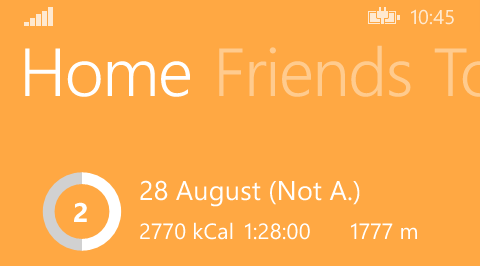
\includegraphics[width=70mm, keepaspectratio]{figures/TabbedPageTitleMissing_wp81.png}\hspace{5mm}
	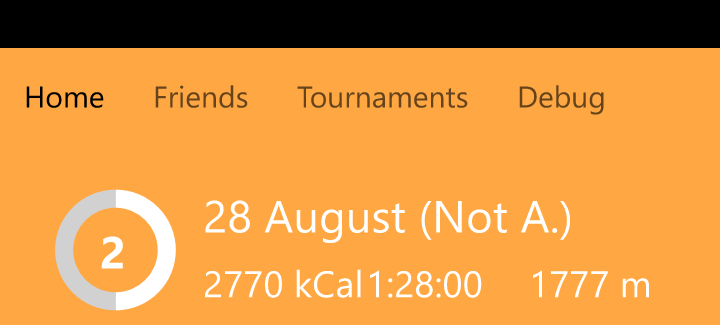
\includegraphics[width=70mm, keepaspectratio]{figures/TabbedPageTitleMissing_wp10.png}\hspace{5mm}
	\caption{Hi�nyz� TabbedPage oldalc�m Windows Phone 8.1 �s Windows 10 Mobile rendszereken} 
	\label{fig:TabbedPageTitleMissing}
\end{figure}
\FloatBarrier

A probl�ma megold�s�ra el�sz�r �t�ll�tottam a platformspecifikus projektekben a Xamarin NuGet verzi�t 2.0.1.6505-re, ezzel a c�mprobl�ma megsz�nt (\figref{TabbedPageTitleOk} �bra).
\begin{figure}[!h]
	\centering
	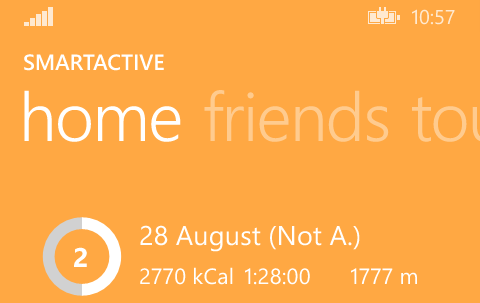
\includegraphics[width=70mm, keepaspectratio]{figures/TabbedPageTitleOk_wp81.png}\hspace{5mm}
	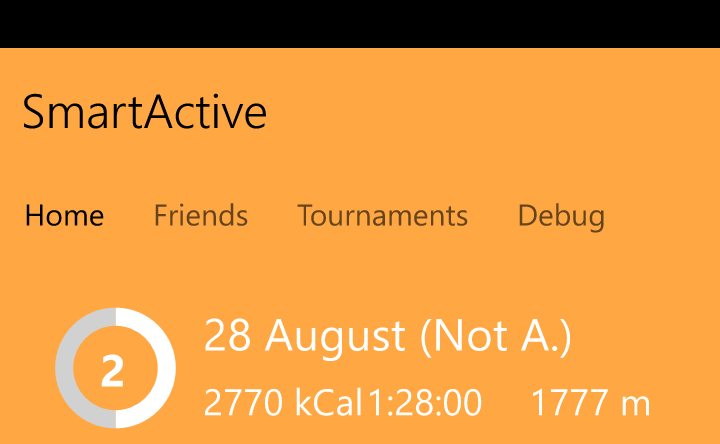
\includegraphics[width=70mm, keepaspectratio]{figures/TabbedPageTitleOk_wp10.png}\hspace{5mm}
	\caption{Helyes TabbedPage oldalc�m Windows Phone 8.1 �s Windows 10 Mobile rendszereken} 
	\label{fig:TabbedPageTitleOk}
\end{figure}
\linebreak K�zi tesztel�skor azonban azt tapasztaltam, hogy Windows Phone 8.1-en ez a keretrendszer-verzi� hib�t tartalmaz a keres�s�v elemben, a keres�sz� helyett �res sztringet ad vissza lek�rdez�skor. Az id�k�zben kiadott 2.2.0.31-es Xamarin verzi� v�ltoztat�sai k�z�tt szerepel a TabbedPage oldalc�m�nek �jb�li bevezet�se a k�t platformon, �gy azokat friss�tettem.
Ekkor a keres�s�v �jra megfelel�en m�k�d�tt Windows Phone 8.1-en, viszont az oldalc�m bet�t�pusa t�l nagy lett (\figref{TabbedPageTitleTooBig} �bra), de �gy d�nt�ttem, a m�k�d� keres�s�v fontosabb, ez�rt enn�l a verzi�n�l maradtam.
Windows Mobile 10-en a friss�t�st�l elt�nt a gombok kerete (\figref{ButtonFrameMissing} �bra).
A gombkeret explicit meghat�roz�s�val sem siker�lt helyre �ll�tanom azokat, �gy v�g�l vissza�lltam a 2.0.1.6505-�s verzi�ra ezen a platformon.

Ezekb�l is l�tszik, hogy a Xamarin egy nagyon �jszer� �s dinamikusan fejl�d� keretrendszer, illetve a multi-platform technol�gia sz�mos kih�v�st ny�jt m�g.
\begin{figure}[!h]
	\centering
	\begin{floatrow}
		\ffigbox {
			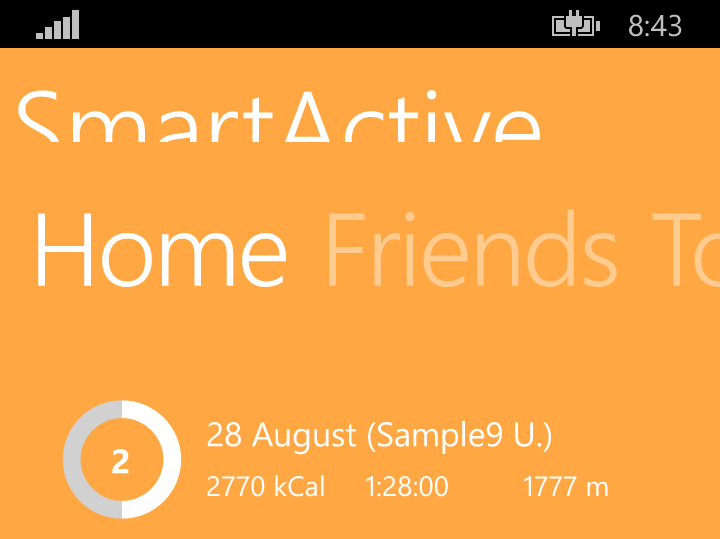
\includegraphics[width=70mm, keepaspectratio]{figures/TabbedPageTitleTooBig_wp81.png}\hspace{5mm}
		}
		{
			\caption{T�l nagy TabbedPage oldalc�m}
			\label{fig:TabbedPageTitleTooBig}
		}
		\ffigbox {
			
\includegraphics[width=55mm]{figures/ButtonFrameMissing_wp10.png}\\\vspace{3mm}
			
\includegraphics[width=55mm]{figures/ButtonFrameOk_wp10.png}\hspace{50mm}
		}
		{
			\caption{Hi�nyz� �s megl�v� gombkeret}
			\label{fig:ButtonFrameMissing}
		}
	\end{floatrow}
\end{figure}
\FloatBarrier
%----------------------------------------------------------------------------
\subsection{Elemek elhelyez�se az oldalakon}\label{sect:ElementPlacement}
%----------------------------------------------------------------------------
A legt�bb oldalt�pus rendelkezik egy \textit{Content} tagv�ltoz�val, aminek a t�pusa\linebreak \textit{Xamarin.Forms.View}.
Ez az oszt�ly az �se az �sszes megjelen�thet� vizu�lis �s vez�rl�elemnek.
Mivel oldalank�nt csak egy Content tag van, ha t�bb elemet k�v�nunk elhelyezni, egy elrendez�si kont�nert (angolul layout) kell haszn�lni, amibe azt�n a t�bbi elem ker�lhet.
Mivel ezek az oszt�lyok is Xamarin View-k, ez�rt tetsz�leges m�lys�gben �s vari�ci�ban �gyazhat�ak egym�sba komplex elrendez�sek megval�s�t�s�ra.
A keretrendszer 9 kont�nert k�n�l \cite{XamarinLayouts}, ezek k�z�l �n a GridLayout, StackLayout �s ScrollView oszt�lyokat haszn�ltam.

A \textit{StackLayout} a legegyszer�bb elrendez�si forma.
Be�ll�t�st�l f�gg�en f�gg�legesen vagy v�zszintesen helyezi egym�s mell� a benne t�rolt elemeket, ezen t�l csak az elemek k�z�tti t�rk�z �ll�that�.

\textit{GridLayout} haszn�latakor meghat�rozhatunk egy r�csszerkezetet annak sorainak �s oszlopainak sz�m�val.
Megadhatjuk a sorok �s oszlopok m�reteit, ak�r a teljes rendelkez�sre �ll� ter�let sz�zal�kos eloszl�s�ban is.
Ez k�l�n�sen hasznos a grafikusfel�let-programoz�sban kezd�knek, akik sz�m�ra a pixelekben t�rt�n� pozicion�l�s igen neh�zkes.

A \textit{ScrollView} list�k megjelen�t�s�re haszn�lhat�. A cella kin�zet�t sablonnal\linebreak hat�rozzuk meg, adatait adatk�t�sb�l nyeri (l�sd \sectref{XamlDataBinding} pont), amihez\linebreak tipikusan rendezett list�t haszn�lnak.
A list�k k�t�s�ben seg�t a\linebreak\textit{System.Collections.ObjectModel.ObservableCollection<T>} sablonoszt�ly, mert ennek m�veletei az elemeken automatikusan friss�t�si mechanizmust v�ltanak ki.

Az ObservableCollection-�k haszn�latakor k�t gyakran, de v�letlenszer�en felbukkan� hib�val tal�lkoztam. 
Az egyik, hogy a ScrollView a v�rttal ellent�tben nem friss�l. 
Ennek megold�sak�nt az objektumot csak a fut�s kezdetekor inicializ�lom, majd m�g teljes friss�t�skor sem cser�lem le azt egy m�sik oszt�lyp�ld�nyra, hanem az objektum \textit{Clear()}, majd \textit{Add()} met�dusait haszn�lom az �j elemek beilleszt�s�re. Ennek h�tter�ben az �ll, hogy az objektum cser�j�vel felbomlanak a megl�v� adatk�t�sek, amik meg�j�t�s�ra nincs m�d \cite{ObservableCollectionMistakes}.\linebreak
A m�sik probl�ma a megjelen�tett lista r�szleges friss�l�se volt.
Ennek megold�sakor der�lt f�ny az adatk�t�s sz�lbiztoss�g�nak hi�ny�ra (l�sd \sectref{AsyncMechanisms} pont).
Az adatok sz�r�s�hez �s rendez�s�hez LINQ\footnote{A Language-Integrated Query k�nyvt�r hat�kony kollekci�manipul�l�si funkci�kat ny�jt szinte b�rmilyen adatforr�shoz \cite{MicrosoftLINQ}.} lek�rdez�seket haszn�l a program, amik a \Csharp~nyelv \textit{yield return} funkci�j�t kihaszn�lva el�re nem, hanem csak akkor hozz�k l�tre az eredm�nyhalmaz-kollekci�t, amikor azon iter�lni kezd�nk.
Ez a mechanizmus olyan �llapot id�zhet el�, amikor a grafikus fel�let ScrollView-ja m�g az adatk�t�tt ObservableCollection friss�t�s�nek befejez�se el�tt v�grehajtja a megjelen�tett lista friss�t�s�t.
Ennek az �llapotnak az elker�l�s�re az eredm�nyhalmazt m�g a h�tt�rsz�lban egy \textit{System.Collections.Generic.List<T>} objektumba enumer�lom, �s fel�lvizsg�lva az alkalmaz�s sz�lkezel�s�t m�dos�t�sokat eszk�z�ltem, hogy az adatk�t�sek friss�t�se mindig az utols� l�p�s legyen az adott m�veletsorban.

Az applik�ci�ban haszn�lt diagramokat kezdetben a ny�lt forr�sk�d� OxyPlot \cite{OxyPlot} csomaggal kezdtem megval�s�tani.
Ez a rendszer st�lusozhat�s�gi k�pess�geiben nem felelt meg a k�vetelm�nyeknek, valamint s�lyos stabilit�si probl�m�kkal rendelkezik Windows 10 Mobile-on, ez�rt a Syncfusion Essential Studio for Xamarin \cite{SyncFusionXamarin} programcsomagra v�ltottam.
A Syncfusion k�nyvt�rai tiszt�n XAML-ben, adatk�t�ssel programozhat�ak, �gy a diagramok integr�l�sa �s st�lusoz�sa gyors �s probl�mamentes volt.

%----------------------------------------------------------------------------
\subsection{St�lusoz�s}\label{sect:Styling}
%----------------------------------------------------------------------------
A Xamarin.Forms vizu�lis elemei k�l�n be�ll�t�s n�lk�l az oper�ci�s rendszer alap�rtelmezett st�lus�val jelennek meg.
Lehet�s�g van azonban az egyes grafikuselem-t�pusokhoz XAML st�lusdefin�ci�k �r�s�ra, amivel biztos�that� az alkalmaz�s egys�ges kin�zete \cite{XamarinStyles}.

A st�lus lehet adott grafikus elemhez �rott vagy glob�lisan el�rhet�, illetve explicit vagy implicit.
Explicit st�lusokn�l az objektum \textit{Style} tulajdons�g�t hozz� kell k�tni a st�lushoz, m�g az implicit st�lusdefin�ci� automatikusan �rv�nyes�tve lesz minden olyan objektumra, aminek t�pus�t az implicit st�lus c�lozza (hacsak fel�l nem b�r�ljuk azt az objektumon).
Az implicit st�lusokkal nem siker�lt l�that� eredm�nyt el�rnem, ez�rt az alkalmaz�s explicit st�lusokat haszn�l.

A k�l�nb�z� platformokon haszn�lt st�lusoz�si aj�nl�sok k�l�nb�z� bet�m�retekkel dolgoznak, illetve az elemek alap kin�zete is jelent�sen k�l�nb�zhet, az alkalmaz�s kin�zet�t ehhez igaz�tani igen k�r�lm�nyes.
Ezen egyszer�s�t a XAML \textit{x:Static} le�r�b�v�tm�nye, amivel lehets�ges \Csharp-ban deklar�lt publikus statikus v�ltoz�kat adatk�tni.
A f�ggel�k \sectref{xStaticExample} pontj�ban l�v� k�dr�szletek szeml�ltetik, ahogy a \textit{Device.OnPlatform()} f�ggv�ny a k�v�nt megjelen�st biztos�t� �rt�kre �ll�tja a statikus v�ltoz�t, majd a XAML k�d XML n�vt�rk�nt (\textit{local}) hivatkozza a \Csharp~n�vteret, �s a statikus v�ltoz� �rt�k�t k�ti a st�lus bet�m�ret tulajdons�g�hoz.

Az x:Static haszn�lat�val nem csak st�lustulajdons�gokhoz k�thet�nk statikus v�ltoz�kat. A gombok alap�rtelmezett kin�zete iOS rendszeren nem megfelel� az alkalmaz�s sz�ns�m�j�hoz, mert nem k�l�nb�zik az egyszer� sz�vegt�l (\figref{ButtonDefaultIOS} �bra).
Keret hozz�ad�s�val azonban a sz�veg t�l k�zel helyezkedik el a kerethez (\figref{ButtonFrameIOS} �bra).
Megold�sul csak enn�l a platformn�l a sz�veg elej�re �s v�g�re is egy-egy sz�k�zt raktam a megfelel� megjelen�shez (\figref{ButtonFrameAndTextIOS} �bra). A kapcsol�d� k�dr�szletek a f�ggel�k \sectref{xStaticButtonExample} pontj�ban tal�lhat�k.

\begin{figure}[!h]
	\centering
	\begin{floatrow}
		\ffigbox {
			
\includegraphics[keepaspectratio]{figures/IOSButtonDefault.png}
		}
		{
			\caption{iOS gomb alap�rtelmezett kin�zete}
			\label{fig:ButtonDefaultIOS}
		}
		\ffigbox {
			
\includegraphics[keepaspectratio]{figures/IOSButtonFrame.png}
		}
		{
			\caption{iOS gomb kerettel}
			\label{fig:ButtonFrameIOS}
		}
	\end{floatrow}
	\vspace{3mm}
	\begin{floatrow}
		\ffigbox {
			
\includegraphics[keepaspectratio]{figures/IOSButtonFrameAndText.png}
		}
		{
			\caption{iOS gomb platformspecifikus sz�veggel �s kerettel}
			\label{fig:ButtonFrameAndTextIOS}
		}
	\end{floatrow}
\end{figure}
\FloatBarrier

A st�lusoz�s folyam�n is probl�m�kba �tk�ztem a TabbedPage oszt�llyal.
A \figref{TabbedPageTitleOk} �br�n l�that�, hogy Windows 10 Mobile rendszeren az oldalc�m �s a f�lek nevei fekete sz�n�ek.
A \figref{TabBarWrongColorAndroid} �bra pedig a f�ls�v-st�lusoz�s hi�ny�t mutatja Android oper�ci�s rendszeren.
Mindk�t probl�ma arra vezethet� vissza, hogy jelenleg a TabbedPage oszt�ly nem rendelkezik tulajdons�gokkal a f�ls�v st�lusoz�s�ra.
A 2.0-�s verzi� el�tt ez lehets�ges volt a \textit{TabBar} tagv�ltoz� megfelel� tulajdons�gainak be�ll�t�s�val, azonban ezt a funkci�t elt�vol�tott�k.
A ny�lt forr�sk�d� Xamarin-Forms-Labs \cite{XamarinFormsLabs} projekt kor�bban egy ker�l� megold�st ny�jtott \textit{ExtendedTabbedPage} oszt�ly�val, azonban 2015 folyam�n a st�lusoz�s funkci� hat�stalann� v�lt, m�ra pedig a forr�sk�d is t�r�lve lett a projekt GitHub t�rhely�r�l.
Ezek miatt a st�lushib�k a v�gleges alkalmaz�sban is jelen vannak.
\begin{figure}[!h]
	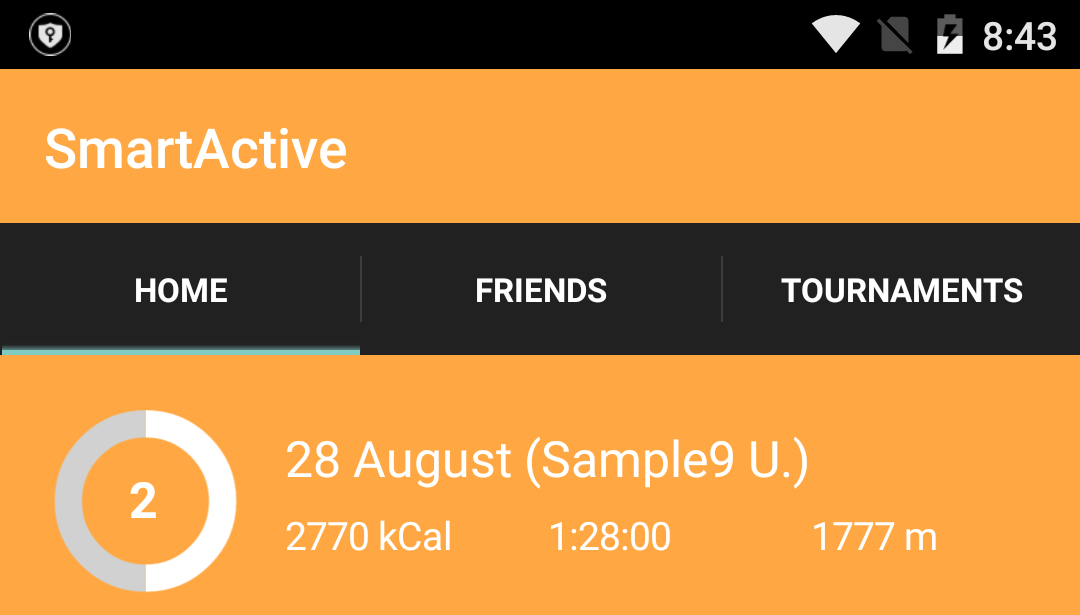
\includegraphics[width=70mm, keepaspectratio]{figures/TabBarWrongColorAndroid.png}
	\caption{A st�lushoz nem illeszked� f�ls�v Android rendszeren}
	\label{fig:TabBarWrongColorAndroid}
\end{figure}

%----------------------------------------------------------------------------
\section{Az alkalmaz�s tesztel�se}
%----------------------------------------------------------------------------
A tesztel�si feladatokon t�l m�r az implement�ci� sor�n szerettem volna cs�kkenteni a hib�k sz�m�t, ez�rt a munka megkezd�sekor telep�tettem a JetBrains Resharpert \cite{ReSharper}.
Ez egy gazdag funkcionalit�s� automatikus k�dkieg�sz�t� �s folyamatos fut�s� statikushiba-keres� program.
Nem csak szintaktikai, de egyes szemantikai hib�kat is k�pes jelezni, valamint javaslatokat tesz k�dr�szletek optimaliz�l�si lehet�s�geire, ezzel jav�tva a k�dmin�s�get.

%----------------------------------------------------------------------------
\subsection{Unit tesztek}\label{sect:UnitTests}
%----------------------------------------------------------------------------
A unit tesztek k�sz�t�se sor�n az alkalmaz�s funkci�inak f�ggv�nyszint� m�k�d�s�t ellen�rizz�k pozit�v �s negat�v tesztesetekkel.
M�sk�pp fogalmazva a f�ggv�nyeknek szab�lyos vagy szab�lytalan inputot adunk, �s a tesztben azt ellen�rizz�k, hogy a bemenetet a v�rt m�don kezeli-e a f�ggv�ny.
A unit tesztek hasznoss�g�t bizony�tja a tesztk�zpont� fejleszt�s (Test Driven Development, TDD) megjelen�se �s t�rnyer�se is.
A TDD-ben az oszt�lystrukt�ra megtervez�se �s v�z�nak elk�sz�t�se ut�n el�sz�r az �tfog� unit tesztek k�sz�lnek el, csak ezut�n t�rt�nik meg a funkci�k implement�ci�ja.

A .NET keretrendszerben �rt k�dok unit tesztel�s�re m�ra kv�zi szabv�nny� v�lt a ny�lt forr�sk�d� NUnit \cite{NUnitHome}.
A rendszernek l�tezik Xamarinhoz optimaliz�lt verzi�ja, ekkor a tesztfuttat� k�rnyezet egy, a telefonra telep�l� program, ami elind�t�sakor lefuttatja a teszteket, majd egy �sszefoglal�t ny�jt az eredm�nyekr�l (\figref{NunitMobileRun} �bra).
\begin{figure}[!h]
	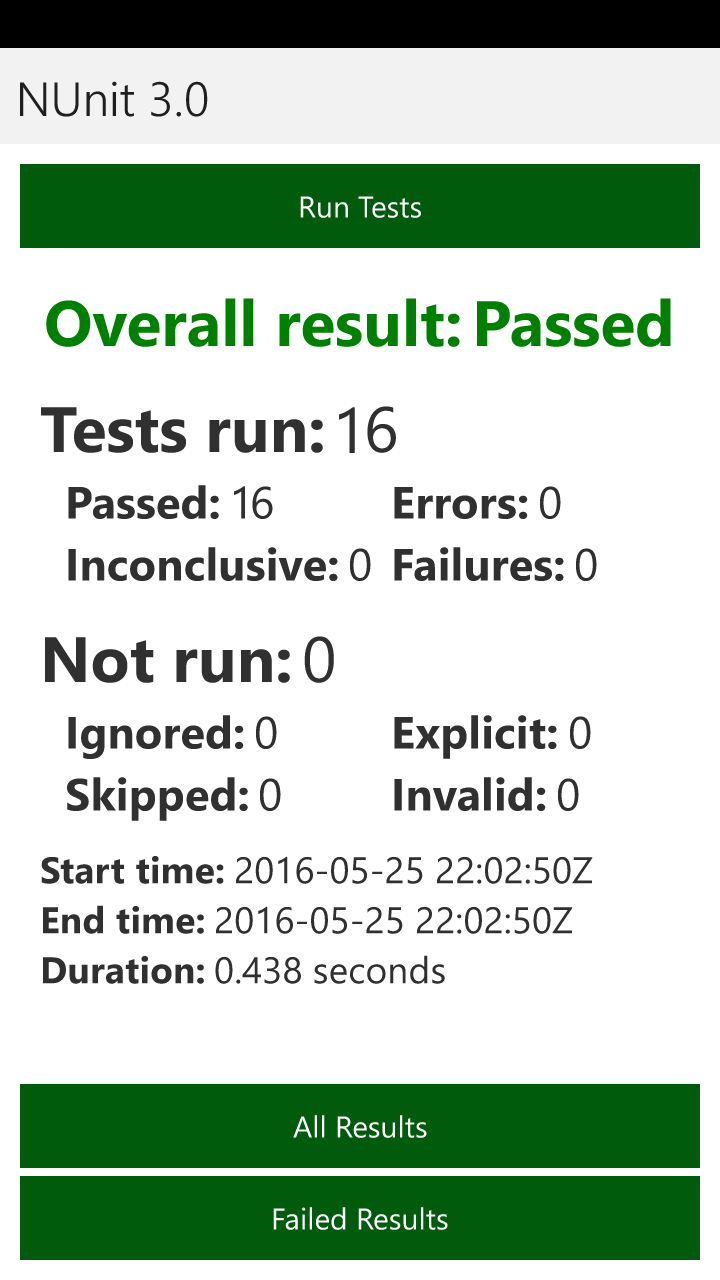
\includegraphics[width=65mm, keepaspectratio]{figures/Nunit_wp10.png}
	\caption{Egy NUnit tesztfut�s eredm�nye Windows 10 Mobile-on}
	\label{fig:NunitMobileRun}
\end{figure}

A hordozhat� oszt�lyk�nyvt�rbeli k�d Visual Studioban futtathat� tesztel�s�re l�trehoztam egy asztali .NET alkalmaz�st c�lz� projektet, a tesztk�dot pedig egy megosztott projektbe helyeztem. �gy m�r haszn�lhat� tetsz�leges unittesztfuttat�-k�rnyezet a tesztek Visual Studioban t�rt�n� futtat�s�ra �s ki�rt�kel�s�re.

Erre a c�lra a JetBrains dotCover \cite{DotCover} futtat�k�rnyezetet v�lasztottam, ami a teszteredm�nyek megjelen�t�s�n t�l k�pes k�dlefedetts�g-vizsg�latra is, azaz megmutatja, hogy a tesztek sor�n a term�kk�d mely sorai ker�ltek lefut�sra.
Egy ilyen vizsg�lat eredm�ny�t mutatja a \figref{DotCoverResult} �bra. Min�l t�bb k�dot fed�nk le min�l sokr�t�bb tesztekkel, ann�l biztosabbak lehet�nk, hogy az applik�ci� az elv�rt viselked�st produk�lja sz�ls�s�ges k�r�lm�nyek k�z�tt is.
\begin{figure}[!h]
	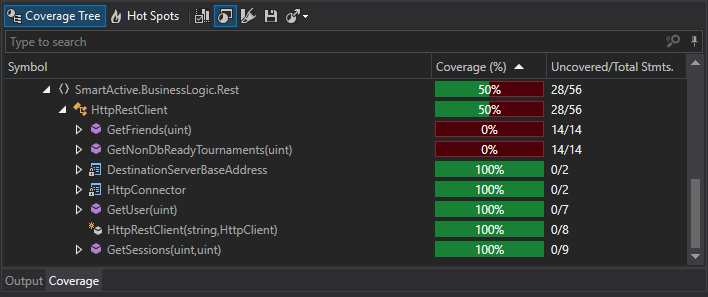
\includegraphics[width=150mm, keepaspectratio]{figures/TestCoverage.png}
	\caption{Egy dotCover k�dlefedetts�g-vizsg�lat eredm�nye a HttpRestClient oszt�lyon}
	\label{fig:DotCoverResult}
\end{figure}

Az applik�ci�hoz 16 unit tesztet k�sz�tettem, amik az �zleti logika viselked�s�t ellen�rzik.
NUnit tesztekkel �nmag�ban a grafikus fel�let m�k�d�se nem ellen�rizhet�.
Erre a Xamarin a TestCloud term�k�t k�n�lja, amihez a Xamarin.UITest k�nyvt�r haszn�lat�val lehet �rni teszteket.
Ilyen teszteket nem �llt m�domban k�sz�teni, mert a Xamarin Student Partner Programban\footnote{A program honlapja: \url{https://www.xamarin.com/student}} ig�nyelt TestCloud hozz�f�r�s-k�relmemet nem b�r�lt�k el kell� id�ben.

%----------------------------------------------------------------------------
\subsection{Manu�lis tesztek}
%----------------------------------------------------------------------------
A grafikus alkalmaz�sok fejleszt�se megk�veteli az �rott k�d folyamatos ellen�rz�s�t.
A Xamarin.Forms a Microsoft WPF-fel szemben m�g nem rendelkezik �gynevezett betekint�n�zet funkci�val, azaz csak �gy l�that� a vizu�lis elemek implement�ci�j�nak eredm�nye, ha az alkalmaz�st leford�tjuk, majd futtatjuk p�ld�ul egy emul�torban (l�sd \sectref{EmulatorUsage} pont).
Mivel az applik�ci� multi-platform, ez�rt minden ellen�rz�st n�gy emul�torban kellett elv�geznem, hogy a platformspecifikus hib�kra is f�ny der�lj�n.

A fejleszt�s sor�n k�t ismer�s�met k�rtem meg, hogy tesztelj�k az alkalmaz�st az emul�torokban.
�k funkcion�lis gondokat nem, csak platformspecifikus megjelen�si hib�kat jeleztek, mint p�ld�ul kil�g� sz�vegek, vagy a TabbedPage oszt�ly azon hib�ja, amit a \sectref{PageTypes} pontban r�szletesen ismertetettem.
Ezeket a hib�kat - a lehet�s�gekhez m�rten - jav�tottam.
Az alkalmaz�s v�gleges androidos verzi�j�t val�di telefonon is teszteltem.
Egy Android 6.0 "Marshmallow" rendszert futtat� LG G3 (D855) k�sz�l�kre telep�tettem az appot.
Az applik�ci� a v�rtaknak megfelel�en viselkedett, nem mutatott elt�r�st az emul�torban tapasztaltakhoz k�pest.
% !TeX encoding = ISO-8859-2
%----------------------------------------------------------------------------
\chapter{Ismeretlen dokumentumt�r: Webt�rk�pez�s}\label{sect:webmapping}
%----------------------------------------------------------------------------
A feladat sor�n rendelkez�semre bocs�tottak egy 700.000 webc�met tartalmaz� .csv f�jlt. Itt minden URL-hez meg volt adva egy vagy t�bb kateg�ria, ami alapj�n a weboldal tartalm�t m�r egy�b m�dszerek seg�ts�g�vel jellemezt�k. �sszesen t�bb mint �tven kateg�ri�ra osztotta fel a c�meket a f�jl, pl.: oktat�s, web�ruh�z, k�z�ss�gi oldal, h�roldal, t�rhely, stb. Ezt haszn�ltam fel az �ltalam el��ll�tott kateg�ri�k ellen�rz�s�re.

%----------------------------------------------------------------------------
\section{Param�terek}
%----------------------------------------------------------------------------
Az elemz�s sor�n a k�vetkez� inform�ci�kat szerettem volna megtudni egy weboldalr�l:
\begin{itemize}
	\item Mik a leggyakoribb, j�l elk�l�n�thet� t�mak�r�k? 
	\item H�ny t�mak�rre lehet hat�konyan bekategoriz�lni a weboldalakat? 
	\item Milyen nyelv�ek az oldalak?
	\item Kinyerhet�ek-e a weboldal tartalm�ra legjellemz�bb kifejez�sek?
\end{itemize}

%----------------------------------------------------------------------------
\section{Funkci�k tervez�se �s megval�s�t�s}
%----------------------------------------------------------------------------
A tervez�s f�zisban a m�r ismertetett m�dszereket vettem alapul. A webelemz�s sor�n a k�vetkez� l�p�seket terveztem meg, majd implement�ltam:
\begin{enumerate}
	\item F�zis: \textbf{linkek form�z�sa}: ebben a f�zisban a felhaszn�l� �ltal megadott URL c�meket rendezem �ssze, �s t�rolom el olyan form�ban, hogy a webcrawler-em k�pes legyen azokat bej�rni. A linkek megad�sa sor�n egy sz�veges beviteli mez�be �rhat�ak be az linkek. Ezt az alkalmaz�s dinamikusan form�zza, majd pedig JSON objektumk�nt lementi.
	\item F�zis: \textbf{Dokumentumt�r kialak�t�sa}: ebben a f�zisban ind�tom el az URL lista bej�r�s�t a meg�rt Spider-rel. Seg�ts�g�vel elk�l�n�tett dokumentumokat hozok l�tre, melyek tartalmazz�k az adott internetes c�mek m�g�tt rejl� weboldalak sz�veges tartalm�t.
	\item F�zis: \textbf{Webelemz�s}: ebben a f�zisban t�rt�nik meg a Topic-modelling elj�r�s futtat�sa, mely sor�n megpr�b�lom �sszehasonl�tani a kiolvasott weboldalak tartalm�t, �s Klaszterez�si elj�r�s seg�ts�g�vel kateg�ri�kra bontom �ket. 
\end{enumerate}

%----------------------------------------------------------------------------
\subsection{Dokumentumt�r kialak�t�sa}
%----------------------------------------------------------------------------
A dokumentumt�r elk�sz�t�s�re az �ltalam �rt Spider-t haszn�ltam fel. 
Ez az alkalmaz�s legink�bb id�ig�nyes l�p�se. A fut�st megk�nny�tend�, egyszerre t�bb p�ld�ny is futtathat�, felosztva k�z�tt�k a bej�rand� webtartom�nyt.
A Spider-t �gy konfigur�ltam fel, hogy hib�s vagy nem l�tez� weboldal eset�n ne pr�b�lkozzon �jra a DNS lek�rdez�ssel \cite{DNS}, illetve a nagyon lassan let�lt�d� weboldalak eset�n �ll�tsa meg a let�lt�st �s ugorjon tov�bb. Ezek n�lk�l ezer link let�lt�se t�bb �r�t vett ig�nybe, �gy csak n�h�ny percet.
A spider a k�vetkez� algoritmus szerint m�k�dik:
\begin{enumerate}
	\item A DOM-b�l kiv�lasztja a <body> tag k�z�tt l�v� tartalmat.
	\item Kit�rli a dokumentumban tal�lhat� sort�r�seket.
	\item Kit�rli a dokumentumb�l a <script> �s <style> tag-ek k�z�tt l�v� tartalmat, ez sz�munkra nem hordoz inform�ci�t.
	\item Kit�rli a dokumentumban tal�lhat� egy�b HTML tag-eket, a marad�k sz�veges tartalmat pedig �sszef�zi.
\end{enumerate}

Minden dokumentumhoz let�roltam egy egyedi azonos�t�t, az eredeti URL c�met �s a Google nyelvdetekt�l� algoritmus�nak fut�si eredm�ny�t. 

%----------------------------------------------------------------------------
\subsection{Webelemz�s}
%----------------------------------------------------------------------------
A dokumentumok klaszterez�s�t v�geztem el ebben a modulban. Alapj�ul szolg�l a kor�bban ismertetett sz�vegb�ny�szati modul, ezt fejlesztettem tov�bb. Az algoritmus fut�sa a k�vetkez� l�p�sekb�l �ll:
\begin{enumerate}
	\item Az el�z� l�p�sben let�rolt �sszes dokumentumot szavakra bontom, szavaikat STOP-sz�t�ramat felhaszn�lva megsz�r�m, bel�l�k az �r�sjeleket kitiszt�tom.
	\item El��ll�tom mindegyik sz� el�fordul�si gyakoris�g�t. A leggyakrabban el�fordul� sz� let�rol�sra ker�l az egyes dokumentumhoz, megfigyel�seim alapj�n ez hasznos megfigyel�s a t�mak�r�ket illet�en.
	\item Elk�sz�tem a k�z�s sz�t�rat, let�rolom k�l�n elemz�sekhez.
	\item A dokumentumteret vektoriz�lom, �s tf-idf alapj�n s�lyozom.
	\item A s�lyozott vektorteret LSI model szerint 2, 4, 8 �s 12 dimenzi�s vetkort�rr� reduk�lom.
	\item A l�trej�tt modell-ben topic-modelling elemz�st futtatok, �s a l�trej�v� t�mak�r�k legjellemz�bb szavait kimentem k�l�n.
	\item A dokumentumok mindegyik�t besorolom a hozz� legk�zelebb es� t�mak�r egyik�be.
\end{enumerate}

%----------------------------------------------------------------------------
\subsection{Felhaszn�l�i fel�let}
%----------------------------------------------------------------------------

A felhaszn�l� \aref{WebmappingGUI} �br�n l�that� fel�letet haszn�lhatja a funkci�k el�r�s�re.

\begin{figure}[!ht]
	\centering
	
\includegraphics[width=120mm, keepaspectratio]{figures/WebmapingGUI.png}
	\caption{Webt�rk�pez� modul kezel�fel�lete} 
	\label{WebmappingGUI}
\end{figure}

A webelemz�s megtekint�se oldalon (\ref{WebmappingGUI2} �bra) els�k�nt a n�gy k�l�nb�z� dimenzi�j� elemz�s �ltal meghat�rozott kateg�ri�k szerepelnek.

\begin{figure}[!ht]
	\centering
	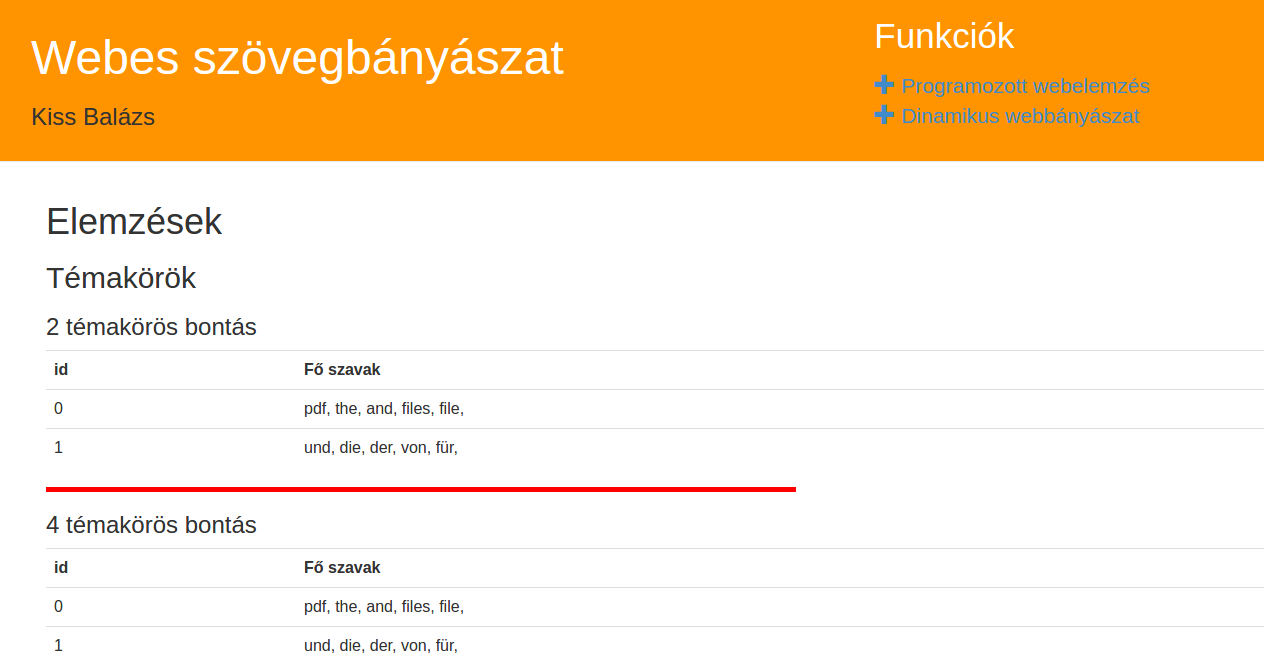
\includegraphics[width=120mm, keepaspectratio]{figures/WebmapingGUI2.png}
	\caption{T�mak�r�k meg�llap�t�sa} 
	\label{WebmappingGUI2}
\end{figure}

A dokumentumok, a meg�llap�tott nyelv, �s a leggyakoribb szavak �s a besorolt kateg�ri�k pedig alattuk (\ref{WebmappingGUI3} �bra).

\begin{figure}[!ht]
	\centering
	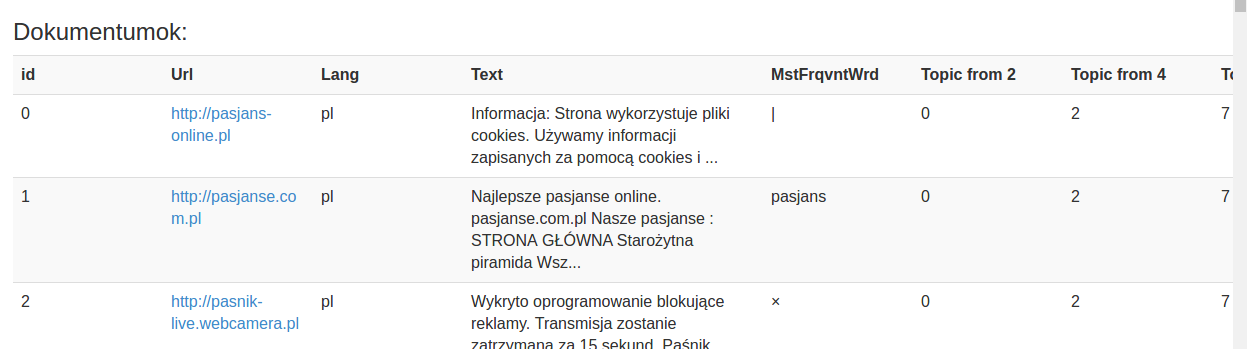
\includegraphics[width=120mm, keepaspectratio]{figures/WebmapingGUI3.png}
	\caption{Dokumentumok �s elemz�s�k eredm�nyei} 
	\label{WebmappingGUI3}
\end{figure}

A feladat sor�n e dokumentumokon v�geztem el t�makutat�st. 

%----------------------------------------------------------------------------
\section{El�zetes eredm�nyek}
%----------------------------------------------------------------------------
Sajnos az adatb�ny�szat egyik jellemz� saj�toss�ga, hogy b�r az algoritmus amit terveztem, elm�letben megfelel�en m�k�dik, a kapott dokumentumt�ren azonban sajnos az eredm�nyek nem voltak kiel�g�t�ek. T�bb probl�ma is felmer�lt a futtat�s sor�n:

\begin{itemize}
	\item \textbf{T�l nagy dokumentumt�r.} A kapott linkgy�jtem�ny �sszesen 375.441 dokumentumot tartalmazott. Ezek mindegyik�b�l �ltal�ban t�bb oldal sz�veg t�lt�d�tt le. Mivel az alkalmaz�son m�k�d�se egy webszerveren val�sul meg, tapasztalataim alapj�n m�r egy p�r t�zezres linklista is jelent�s mem�riahi�nyt okozott a 8 gigabite ram-mal felszerelt g�pen.
	\begin{itemize}
		\item Megold�sk�nt egy 10.000 linkb�l �ll� c�mhalmazra reduk�ltam az elemz�st.
	\end{itemize}
	\item \textbf{T�l nagy kateg�riahalmaz.} A kapott linkekhez �sszesen 52 k�l�nb�z�, legal�bb egy, maximum h�rom c�mk�t rendeltek. Ekkora halmazt szinte lehetelten pontosan reproduk�lni, pl�ne nem az ott meghat�rozott �ltal�nos c�mk�k alapj�n. 
	\begin{itemize}
		\item Megold�sk�nt az elemz�semhez �sszesen n�gy modellt futtattam, 2, 4, 8 �s 12 maxim�lis kateg�ri�t meghat�rozva. Az �ltalam kapott kateg�ri�kban szerepl� dokumentumokon meg tudtam figyelni, hogy van-e szab�lyos minta a c�mk�kben. 
	\end{itemize}

	 A fenti probl�m�kra b�r tal�ltam kompromisszumos megold�st, azonban n�h�ny olyan probl�ma is felmer�lt, amely miatt a feladat �jratervez�se mellett d�nt�ttem.
	 
	 \item \textbf{T�l sok nyelv.} Az elemz�s sor�n a vil�g �sszes t�j�r�l tal�ltam nyelveket. A sz�vegb�ny�szati modul nincsen felv�rtezve azzal a tud�ssal, hogy hasonl� t�m�j� oldalakat nyelvt�l f�ggetlen�l egy csoportba rendezze, hiszen az �ltalam implement�lt m�dszert szinte teljes eg�sz�ben a dokumentumokban tal�lhat� szavakra �p�t. 
	 \begin{itemize}
	 	\item �ltal�nos nyelvi elemz�program �r�sa lenne a megold�s, de ez t�lmutat az egy ember �ltal meg�rhat� projekt hat�rain.
	 \end{itemize}
 
	 \begin{figure}[!ht]
	 	\centering
	 	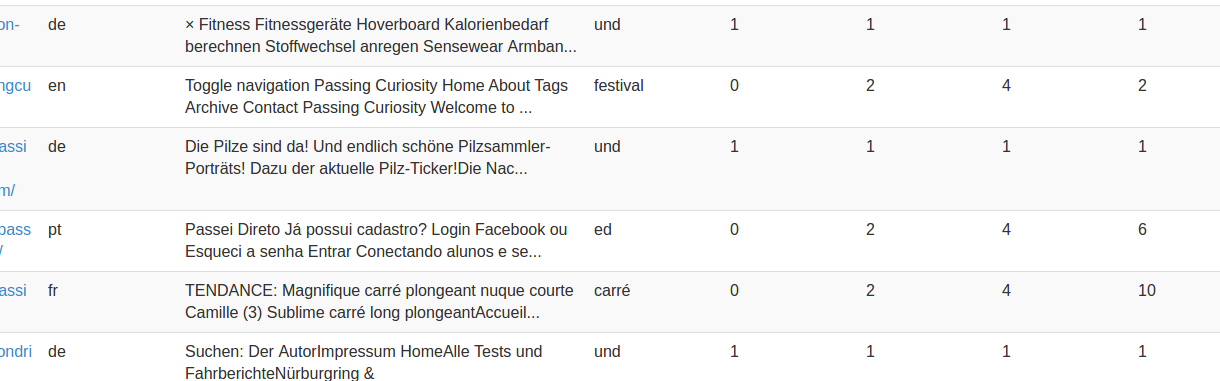
\includegraphics[width=120mm, keepaspectratio]{figures/WebmapingOldResults.png}
	 	\caption{Elemz�s eredm�nye. Balr�l jobbra: weboldal nyelve, kivonat a tartalomb�l, leggyakoribb sz� az oldalon, majd pedig els�k�nt a 2, 4, 8, v�g�l a 12 kateg�ri�s klaszterez�s eredm�nye.} 
	 	\label{WebmapingOldResults}
	 \end{figure}
 
 	\Aref{WebmapingOldResults} �br�n l�that� 1000 weboldal elemz�s�b�l r�szlet. Er�sen �szrevehet�, hogy a nyelvek ment�n alakulnak ki a csoportok. 
 	
 	\item Weboldal tartalma f�lrevezet�. Rengeteg olyan esettel tal�lkoztam, amikor a weboldalon elhelyezked� rekl�mok mennyis�ge nagyobb volt, mint a weboldal hasznos tartalma. Gyakran fordult el�, hogy a gener�lt tartalomban olyan k�dr�szleteket rejtettek el, melynek feladata a keres�motorok f�lrevezet�se. Sok esetben �n magam sem tudtam a nyers HTML tartalom alapj�n kisilabiz�lni, mir�l is sz�lhat az adott oldal. 
 	\item Az oldal k�dja nem utal a tartalomra. A legnagyobb probl�ma a feladattal az volt, hogy az �ltal�nos webcrawler modul nem volt felk�sz�tve a weboldalak saj�toss�gaira. A gyakran el�fordul�, szem�lyre szabott rekl�mokon fel�l olyan oldalr�szletek, mint pl. a cookie-k elfogad�sa, bejelentkez�s, regisztr�ci�, f�oldal bel�p�s �s m�g sz�mos m�s, �ltal�nos weboldal elem, nem utal a weboldal tartalm�ra, m�gis megjelennek a sz�vegben, ez�ltal hamis kateg�ri�kat alkotva. Ezen fel�l egy megjelen�tett weboldal fel�let�nek lehet, hogy nagy r�sz�t egy sz�vegdoboz tesz ki, az a HTML tartalomban azonban csak az oldal tartalm�nak t�red�ke: elmondhat�, hogy egy weboldalt\textbf{ nem lehet a vizu�lis megjelen�t�se n�lk�l hat�konyan bekategoriz�lni.}	 
\end{itemize}

\begin{figure}[!ht]
\centering
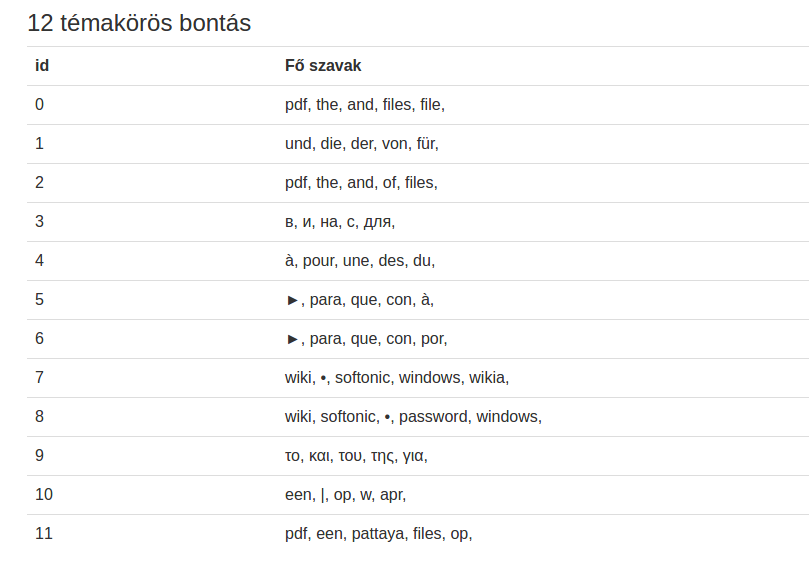
\includegraphics[width=120mm, keepaspectratio]{figures/WebmapingOldResults2.png}
\caption{12 t�mak�r�s klaszterez�s eredm�nye} 
\label{WebmapingOldResults2}
\end{figure}

\Aref{WebmapingOldResults2} �br�n l�that� 1000 weboldal elemz�se sor�n kialakult kateg�ri�k legf�bb szavai. L�tszik, hogy b�r �szrevehet�ek t�mabeli kateg�ri�k, t�bbs�g�ben kezd eluralkodni a nyelvek ment�n kialakul� kategoriz�l�s.

Az elemz�s kimenet�t l�tva a k�vetkez�t �llap�tottam meg:

\begin{itemize}
	\item A program szinte kiv�tel n�lk�l nyelvek ment�n hat�rozza meg a klasztereket. 
	\item A dokumentumok sz�vegez�se k�z�tt akkora �ri�si k�l�nbs�g van, hogy a vektor�rt�kek k�z�tti k�l�nbs�g eleny�sz� - azaz nincsenek j�l elk�l�n�l� kateg�ri�k.
\end{itemize}

%----------------------------------------------------------------------------
\section{�jratervez�s}
%----------------------------------------------------------------------------

A feladathoz eredeti c�lja b�r nem megval�s�that�, m�gis �rdemes meg�llap�tani, mi az a pontos�t�s, ahol m�r haszn�lhat�, hasznos eredm�nyeket kapunk. Ennek �rdek�ben a k�vetkez� m�dos�t�sokat hajtottam v�gre:

\begin{itemize}
\item Tov�bb pontos�tottam a webcrawler modul m�k�d�s�t. Kieg�sz�tettem, hogy m�g t�bb, gyakran el�fordul� tartalmat sz�rj�n ki, �s m�g ink�bb a hasznos tartalmat nyerjem ki a weboldalakr�l.
\item Lesz�k�tettem a m�k�d�st angol nyelvre - teh�t a dokumentumok k�z�l csak azon weboldalak tartalm�ra futtattam le a programot, melyek nyelv�t angolnak �llap�totta meg a nyelvdetekt�l� modul.
\end{itemize}


%----------------------------------------------------------------------------
\section{Angol nyelv� eredm�nyek}
%----------------------------------------------------------------------------
Az �j elemz�s futtat�sa ut�n a k�vetkez� eredm�nyeket tapasztaltam:
\begin{itemize}
	\item Az egynyelv� futtat�s hat�s�ra kik�sz�b�ltem a nyelvkezel�si probl�m�t.
	\item Kis dimenzi� eset�n �ltal�ban k�t nagy klasztert �llap�t meg az algoritmus: 
	\begin{enumerate}
		\item Az egyik kateg�ri�ba tartozik �ltal�ban egy specifikus, de gyakran el�fordul� weboldalt�pus,
		\item a m�sik kateg�ri�ba pedig az �sszes t�bbi oldal.
	\end{enumerate}
	\item Magasabb dimenzi�sz�mok eset�ben is csak n�h�ny j�l elk�l�n�thet� weboldal-t�pus j�n l�tre, nem j�nnek l�tre �jabb, j�l elk�l�n�l� csoportok.  
\end{itemize}

\begin{figure}[!ht]
	\centering
	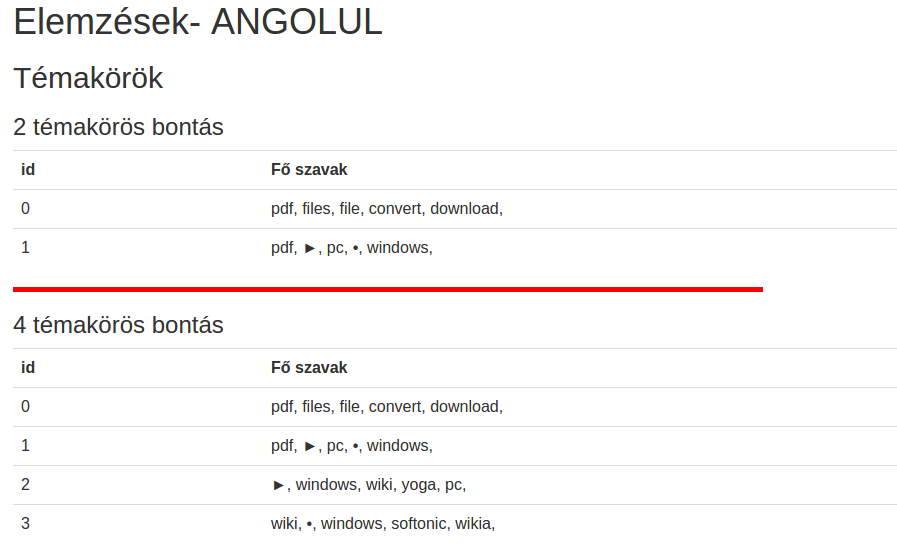
\includegraphics[width=120mm, keepaspectratio]{figures/WebmappingNewResults1.png}
	\caption{Egy angol elemz�s t�mak�rei} 
	\label{WebmappingNewResults1}
\end{figure}

\Aref{WebmappingNewResults1} �br�n l�that�, hogy a k�tdimenzi�s bont�s eset�n, az els� kateg�ria valamilyen f�jllet�lt�s/konvert�l�s t�m�j� oldalakat fog �ssze. 

A m�sodik kateg�ria szavainak s�lyoz�si �rt�keit vizsg�lva az l�tsz�dik, hogy az �sszes sz� egym�shoz k�pest nagyon k�zel van, �rt�k�k szinte azonos. Ebb�l arra k�vetkeztettem, hogy ezek a szavak a "minden m�s" kateg�ri�t k�pviselik.

Tov�bb emelve a dimenzi�sz�mot l�thatjuk, hogy a kor�bbi els� kateg�ri�nk megmarad, az �j kateg�ri�kban viszont tov�bbra is egym�st�l nem t�l j�l elk�l�n�l� csoportok j�nnek l�tre. Ez l�tszik a dokumentumt�ren is(\ref{WebmappingNewResults2} �bra).

\begin{figure}[!ht]
	\centering
	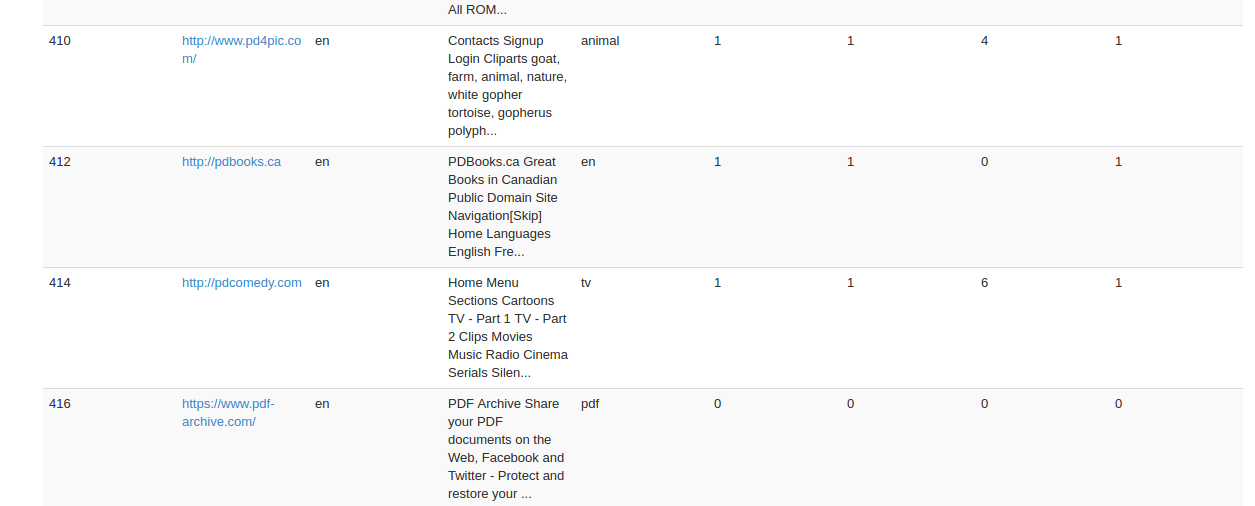
\includegraphics[width=170mm, keepaspectratio]{figures/WebmappingNewResults2.png}
	\caption{Angol elemz�s dokumentum besorol�sai. Balr�l jobbra a k�vetkez� l�that�: weboldal sorsz�ma, URL-je, meg�llap�tott nyelve, sz�veg kivonat, leggyakoribb sz�, majd pedig a 2-4-8-12 dimenzi�s klaszterez�s eredm�nyei.} 
	\label{WebmappingNewResults2}
\end{figure}

Az �br�n l�tszik, hogy a 416-os, online pdf t�rhelyet a "0"-s kateg�ri�ba sorolja a program, m�g az �sszes t�bbi oldalt a m�sik kateg�ri�ba. Magasabb dimenzi�sz�m eset�n �rdemben ez a feloszt�s nem v�ltozik. 

Meg�llap�tottam, hogy az elemz�st a kor�bban eml�tett neh�zs�gek, a webes tartalom zajoss�ga, �s a html tartalom saj�toss�gai miatt ilyen m�rt�kn�l jobban az �ltalam felhaszn�lt eszk�z�kkel pontosabban nem lehet megoldani.

Az elemz�seket akkor lehetne pontosabb eredm�nnyel futtatni, ha sokkal sz�lesebb algoritmikus �s hardveres eszk�zt�r �llna a rendelkez�sre, illetve ha komplex feldolgoz�s�t v�gezn�nk el egy weboldalnak a DOM sz�vegkinyer�se mellett. 

















%----------------------------------------------------------------------------
\chapter{Konkl�zi�, tov�bbviteli lehet�s�gek}
%----------------------------------------------------------------------------
Munk�m sor�n megismerkedtem a Xamarin multi-platform szoftverfejleszt� keretrendszerrel, �s tapasztalatot szereztem egy komplex grafikus alkalmaz�s elk�sz�t�s�ben a\linebreak\Csharp~nyelv, Microsoft fejleszt�eszk�z�k �s korszer� programoz�si paradigm�k haszn�lat�val.
Betekint�st nyertem a unit tesztek k�sz�t�s�be az NUnit keretrendszerrel, �s megtapasztaltam ezen tesztek hasznoss�g�t a k�dmin�s�g szempontj�b�l.

Elk�sz�tettem a SmartActive projekt keret�ben egy mobilalkalmaz�st, ami n�gy k�l�nb�z� mobiloper�ci�s-rendszert t�mogat.
Az alkalmaz�s funkcionalit�sa �s strukt�r�ja minden c�lplatformon megegyezik, ezzel azonos �lm�nyt ny�jtva.
A felhaszn�l� mobilk�sz�l�k�n gyorsan �s hat�konyan hozz�f�rhet a squash sporttev�kenys�g�hez kapcsol�d� statisztik�khoz, valamint a projekt ny�jtotta k�z�ss�gi funkci�kat is ig�nybe veheti: megtekintheti bar�tait, �s bajnoks�gokat szervezhet, amire megh�vhatja ismer�seit.

V�lem�nyem szerint a Xamarin a \Csharp-ban j�ratos fejleszt�k sz�m�ra egy hasznos �s funkcionalit�sban gazdag keretrendszer, haszn�lat�val nincs sz�ks�g a konkurens term�kek nagy r�sz�n�l megk�vetelt webtechnol�gi�k behat� ismeret�re.
Tov�bbi el�nye, hogy a .NET k�nyvt�r jelent�s r�sze haszn�lhat� a k�z�s oszt�lyk�nyvt�rbeli k�dban is.
Ugyanakkor a Xamarin.Forms multi-platform grafikusfel�let-k�nyvt�r m�g fiatals�g�b�l ad�d�an probl�m�kkal �s hi�nyoss�gokkal k�zd, ahogy ezekre munk�mban r�mutattam.

Az alkalmaz�s ut�lagos ki�rt�kel�sekor meg�llap�tottam, hogy a bar�tok hozz�ad�sa funkci�n�l (\sectref{FriendManagement} pont) implement�lt ker�l�megold�s - ami egy bar�trekord l�trehoz�sa a helyi adatb�zisban - helyett haszn�lhattam volna egy JSON f�jlt a dropbox t�rhelyen, ami a felhaszn�l�k list�j�t adja vissza, �s a bejelentkezett felhaszn�l� ebb�l v�laszt.
A webszerver komponens elk�sz�lt�ig ez a m�dos�t�s eszk�z�lhet�, ut�na pedig az alkalmaz�s b�v�thet� k�tir�ny� szinkroniz�l�ssal nem csak a bar�tok hozz�ad�s�n�l, de a bajnoks�gok l�trehoz�s�n�l �s kezel�s�n�l is.
M�g egy hibajav�t�si opci� lehet a TabbedPage oldalc�m�nek platformspecifikus �lt�ntet�se Windows Phone 8.1-en az x:Static le�r�b�v�tm�ny haszn�lat�val (l�sd \sectref{Styling} pont), am�g a Xamarin keretrendszerben ki nem jav�tj�k a \figref{TabbedPageTitleTooBig} �br�n l�that� "t�l nagy oldalc�m-bet�m�ret" hib�t. 

Az applik�ci� diz�jnja a k�s�bbiekben finom�that�, p�ld�ul a hely�rz�k lecser�lhet�k val�s k�pekre, illetve a statisztikai elemek megjelen�se fiatalosabb� tehet� piktogramokkal.
Tov�bb� az applik�ci� a SmartActive projekt el�rehaladt�val �j funkci�kkal b�v�thet�, p�ld�ul a kezdeti tervekben szerepl� p�lyafoglal�si lehet�s�ggel.
Szint�n egy b�v�t�si opci�, hogy az edz�sek inform�ci�i megoszthat�ak legyenek m�s szoci�lis platformokon, mint p�ld�ul Facebook vagy Twitter, valamint import�lhat�ak legyenek bar�tok m�s port�lokr�l, illetve a k�sz�l�k telefonk�nyv�b�l.
A platformt�mogat�s kiterjeszthet� a viselhet� eszk�z�kre, p�ld�ul okos�r�kra, �gy az app ak�r a sportol�s sor�n is szolg�lhat hasznos inform�ci�kkal, �s adatok nyerhet�k ki az �r�ba �p�tett szenzorok seg�ts�g�vel.
Ezzel a fejleszt�ssel a mobilapplik�ci� m�r nem csak fogyaszt�j�v�, hanem szolg�ltat�j�v� is v�lna a sportol�si statisztik�knak.
% !TeX encoding = ISO-8859-2
%----------------------------------------------------------------------------
\chapter{�sszefoglal�s, �rt�kel�s}\label{sect:summary}
%----------------------------------------------------------------------------
A Diplomamunk�m sor�n egy t�bb iter�ci�b�l �s al-feladatokb�l �ll�, komplex webes sz�veg- �s adatb�ny�szati szoftvert k�sz�tettem el.

A m�k�d�shez webes seg�dk�nyvt�rakat, �ltalam �rt algoritmusokat, webcrawlereket �s egy komplett webes keretrendszert haszn�ltam fel. 

A feladat sor�n t�bb elemz�st is elv�geztem, eredm�nyeiket, megfigyel�seimet �rtelmeztem, be�p�tettem a szoftverbe. T�bb l�p�s sor�n jutottam el a v�gs� algoritmusokig, hol a sikeres elemz�seket tov�bbfejlesztve, hol pedig a hib�s elgondol�sokat �jratervezve. 
Elk�sz�tettem egy m�k�d� webalkalmaz�st, amely keretrendszerk�nt t�bbf�le web, adat- �s sz�vegb�ny�szati feladatra is felhaszn�lhat�.

Mindezen eredm�nyeket egy komplex webalkalmaz�sba �ltettem �t, mely seg�ts�g�vel az elemz�sek k�nnyed�n reproduk�lhat�ak. A sz�veg- �s adatb�ny�szati elemz�sek t�bb l�p�se �s a k�d futtat�sa teljesen automatikusan t�rt�nik.

A tervez�s l�p�sei sor�n kialak�tott algoritmusok kimenetei hasznos �s helyes inform�ci�val szolg�lnak. Kutat�saim �s munk�m sor�n a sz�vegb�ny�szat eszk�zeir�l igazoltam, hogy felhaszn�lhat�ak a magyar nyelv� weboldalak eset�ben is. 

A feladat sor�n �sszesen ~3000 sor k�dot �rtam Python, HTML �s egy�b scriptnyelveken. Elm�ly�tettem ismereteimet a Django keretrendszer m�k�d�s�ben, saj�t modult �s fel�leteket terveztem. T�bb seg�dk�nyvt�r �s eszk�z m�k�d�s�t megismertem, elsaj�t�tottam, azokat a feladat megold�s�hoz felhaszn�ltam. 

Az id�m jelent�s h�nyad�t tette ki az adatb�ny�szati modul, �s a sz�vegb�ny�szati l�p�sek megtervez�se, tesztel�se. Az elk�sz�lt programk�dokat alapos tesztel�s ut�n beillesztettem a webalkalmaz�sba. 

%----------------------------------------------------------------------------
\section{Tov�bbfejleszt�si lehet�s�gek}
%----------------------------------------------------------------------------

A webalkalmaz�s tov�bbfejleszt�s�hez az egyik lehets�ges �t a felhaszn�lt adatb�ny�szati elj�r�sok finom�t�sa, f�leg a dinamikus modul eset�ben. M�s adatb�ny�szati elemz�sek kipr�b�l�sa, neur�lis h�l�k alkalmaz�sa, weboldalak k�z�tti egy�b �sszef�gg�sek (pl. egym�sra mutat� linkek, c�mk�k) kutat�sa.

Jelenleg nem l�tezik ingyenesen el�rhet� �s hat�kony magyar sz�t�vez�si elj�r�s - ennek kidolgoz�sa nagyban n�veln� az algoritmus hat�konys�g�t. 

Az elemz�sek testreszabhat�s�g�t n�veln�, ha a k�l�nb�z� webes elemz�sek prec�zi�s param�tereit a felhaszn�l� be�ll�thatn� a webalkalmaz�s fel�let�n. 

A m�sik �tvonal a weboldalakt�l val� f�ggetlened�s: olyan men�pont elk�sz�t�se, amellyel dinamikusan tudunk megadni �j h�rforr�sokat az alkalmaz�s sz�m�ra.

M�sik �tlet, hogy a f�jlok mem�ri�ban, majd pedig a diszken t�rt�n� sz�veges f�jlokk�nt val� t�rol�sa helyett ink�bb egy adatb�zist �p�tsek fel a rendszer m�g�. Az adatt�rol�si r�teg a sk�l�zhat�s�got �s a szoftver feldolgoz� erej�t n�velhetn�, illetve a p�rhuzamos webcrawl eset�n a hardveres sz�k keresztmetszetet cs�kkenten� esetleg egy elosztott rendszerrel t�rt�n� web bej�r�s.

Nagyszab�s� projekt a statikus elemz�sek sor�n, ha t�bb hasonl� oldalra is felk�sz�tj�k az alkalmaz�st, pl. t�bb m�s magyar h�rport�lt is egy�ttesen elemezn�nk, �s ebb�l �llap�tan�nk meg egy nap legfontosabb h�reit - ak�r angol vagy m�s nyelveken is.

A sz�vegb�ny�szati �s topic modelling eszk�z�k k�z�l m�g j� p�r l�tezik, melyeket nem haszn�ltam fel, nem pr�b�ltam ki: ilyen az LSI helyett Random Pojections, RP \cite{gensimMain},  oszt�lyoz�sn�l a k-nn m�dszer, vagy a klaszterez�sn�l a k-medoid klaszterez�s \cite{AbonyiAdatb}, \cite{TikkSzovegb}.

%----------------------------------------------------------------------------
\section{K�sz�netnyilv�n�t�s}
%----------------------------------------------------------------------------
K�sz�n�m konzulensemnek, Nagy G�bornak az �ltal�nos seg�ts�get �s a t�ma mesterk�pz�sen �t�vel� vezet�s�t. Kazi S�ndornak a sz�vegb�ny�szati, python �s \LaTeX\ seg�ts�gny�jt�st. K�sz�n�m a lektor�l�st �kr�s Tam�snak, M�dly M�rknak, M�r�sz D�nielnek �s P�lmai N�r�nak. 





%\listoffigures\addcontentsline{toc}{chapter}{�br�k jegyz�ke}
%\listoftables\addcontentsline{toc}{chapter}{T�bl�zatok jegyz�ke}

\bibliography{mybib}
\addcontentsline{toc}{chapter}{Irodalomjegyz�k}
\bibliographystyle{plain}



\label{page:last}
\end{document}
